\section{Out-of-sample gate weights for every series}\label{app:gates}

\Cref{fig:gates_oos_1,fig:gates_oos_2} show the SMoE's out-of-sample gate probabilities (20-day
moving averages), i.e.\ the regime weights the model actually used when forecasting. They are
computed from the same forecasts that enter all evaluation tables and are therefore free of
look-ahead.

\begin{figure}[p]\centering
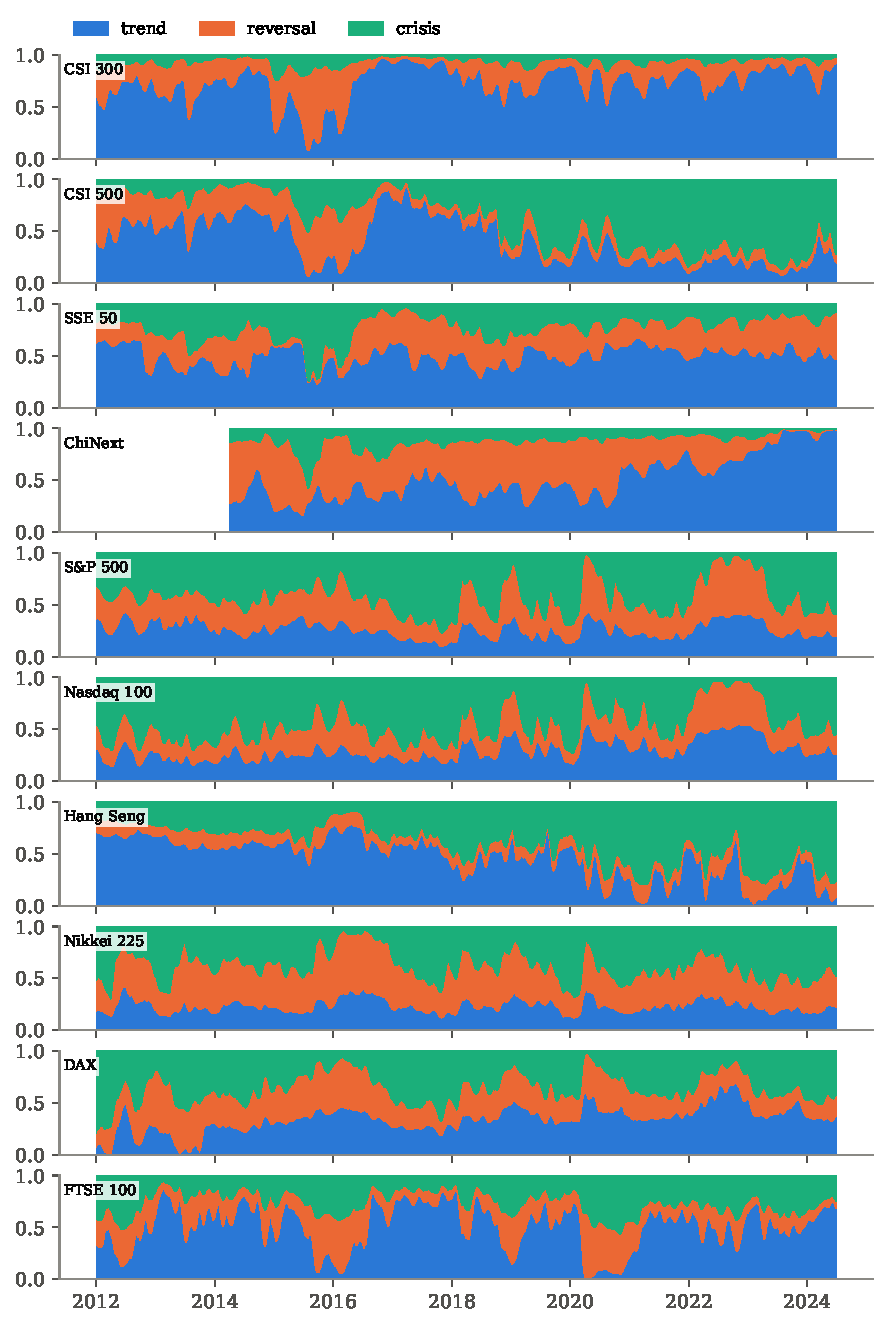
\includegraphics[width=\textwidth,height=0.9\textheight,keepaspectratio]{../results/figures/gates_oos_1.pdf}
\caption{Out-of-sample SMoE gate weights: Chinese and international equity indices.}\label{fig:gates_oos_1}
\end{figure}

\begin{figure}[p]\centering
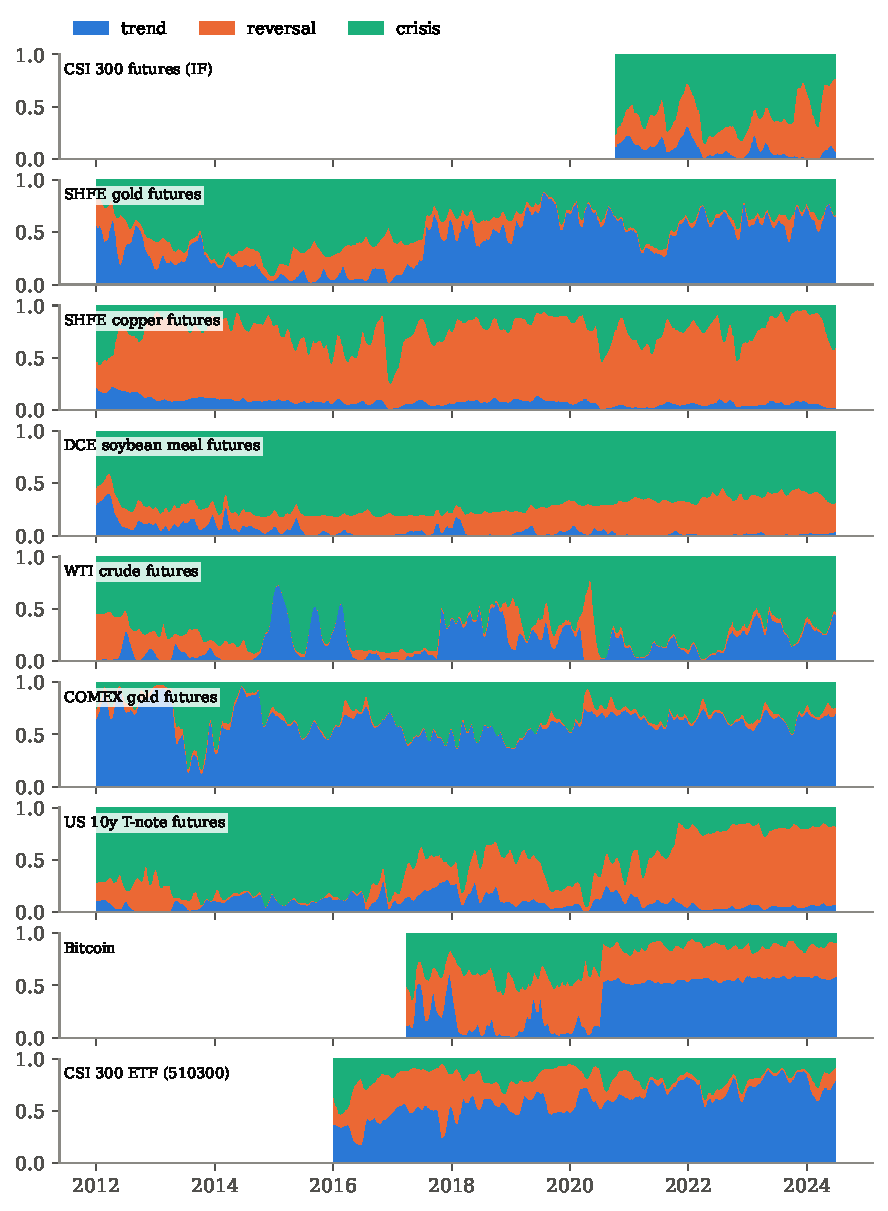
\includegraphics[width=\textwidth,height=0.9\textheight,keepaspectratio]{../results/figures/gates_oos_2.pdf}
\caption{Out-of-sample SMoE gate weights: futures, Bitcoin and the CSI 300 ETF.}\label{fig:gates_oos_2}
\end{figure}

\clearpage
\section{Detailed out-of-sample results by series}\label{app:per-asset}

For every series, the tables report mean losses (lower is better; the best model in bold), the
model-confidence-set $p$-value for log score, the directional hit rate, VaR violation rates with the
Kupiec $p$-value, and the Berkowitz $p$-value of the PIT.

\begin{table}[!htbp]\centering\scriptsize
\caption{Out-of-sample results: CSI 300 ($n=3032$)}\label{tab:asset_csi300}
\begin{adjustbox}{max width=\textwidth}
\begin{tabular}{lrrrrrrrrrrr}
\toprule
Model & NLL & CRPS & QLIKE & FZ5 & Brier & MCS $p$ (NLL) & Hit & Viol 1\% & Viol 5\% & Kupiec 1\% $p$ & Berkowitz $p$\\
\midrule
HistGauss & 1.6889 & 0.7112 & 1.7631 & 1.1842 & 0.2493 & 0.0000 & 0.5261 & 0.0211 & 0.0455 & 0.0000 & 0.0066\\
GARCH-t & 1.5727 & 0.6928 & 1.6004 & 1.0229 & 0.2506 & 0.8920 & 0.5096 & 0.0122 & 0.0485 & 0.2386 & 0.0009\\
AR-GJR-t & 1.5730 & 0.6930 & 1.6007 & 1.0216 & 0.2506 & 0.8290 & 0.5073 & 0.0122 & 0.0482 & 0.2386 & 0.0019\\
Gauss-HAR & 1.5963 & 0.6936 & \textbf{1.5790} & 1.0157 & 0.2502 & 0.0090 & 0.5007 & 0.0191 & 0.0432 & 0.0000 & 0.6238\\
MAR & 1.5783 & 0.6923 & 1.5837 & 1.0300 & 0.2514 & 0.1920 & 0.5125 & 0.0079 & 0.0416 & 0.2313 & 0.6746\\
LSTAR & 1.5722 & 0.6935 & 1.5793 & \textbf{0.9999} & 0.2523 & 0.8920 & 0.5079 & 0.0082 & 0.0429 & 0.3166 & 0.3562\\
MS-AR & 1.6214 & 0.7047 & 1.6868 & 1.0753 & 0.2511 & 0.0000 & 0.4990 & 0.0122 & 0.0402 & 0.2386 & 0.0000\\
XGB-Gauss & 1.6240 & \textbf{0.6904} & 1.6405 & 1.0839 & 0.2492 & 0.0090 & 0.5066 & 0.0297 & 0.0676 & 0.0000 & 0.0000\\
Chronos-Bolt-small & 1.7124 & 0.6982 & 1.8067 & 1.2398 & 0.2506 & 0.0000 & 0.5221 & 0.0359 & 0.0798 & 0.0000 & 0.0000\\
Chronos-Bolt-base & 1.6702 & 0.6964 & 1.7234 & 1.1689 & 0.2500 & 0.0000 & 0.5254 & 0.0307 & 0.0712 & 0.0000 & 0.0000\\
TimesFM-2.5 & 1.6469 & 0.7029 & 1.6648 & 1.1333 & 0.2530 & 0.0000 & 0.4947 & 0.0247 & 0.0590 & 0.0000 & 0.0000\\
Deep-SMoE & \textbf{1.5693} & 0.6908 & 1.5821 & 1.0240 & 0.2496 & 1.0000 & 0.5168 & 0.0102 & 0.0412 & 0.9016 & 0.0200\\
SMoE & 1.5705 & 0.6931 & 1.5831 & 1.0095 & 0.2512 & 0.8920 & 0.5063 & 0.0079 & 0.0416 & 0.2313 & 0.6404\\
\bottomrule
\end{tabular}
\end{adjustbox}
\end{table}
\clearpage
\begin{table}[!htbp]\centering\scriptsize
\caption{Out-of-sample results: CSI 500 ($n=3032$)}\label{tab:asset_csi500}
\begin{adjustbox}{max width=\textwidth}
\begin{tabular}{lrrrrrrrrrrr}
\toprule
Model & NLL & CRPS & QLIKE & FZ5 & Brier & MCS $p$ (NLL) & Hit & Viol 1\% & Viol 5\% & Kupiec 1\% $p$ & Berkowitz $p$\\
\midrule
HistGauss & 1.8334 & 0.8162 & 1.7310 & 1.4251 & 0.2490 & 0.0000 & 0.5234 & 0.0287 & 0.0564 & 0.0000 & 0.0000\\
GARCH-t & 1.7088 & 0.7938 & 1.5461 & 1.2786 & 0.2501 & 0.0010 & 0.5323 & 0.0172 & 0.0623 & 0.0003 & 0.0000\\
AR-GJR-t & 1.7090 & 0.7935 & 1.5473 & 1.2690 & 0.2500 & 0.0010 & 0.5257 & 0.0168 & 0.0623 & 0.0006 & 0.0000\\
Gauss-HAR & 1.7292 & 0.7946 & 1.5230 & 1.2580 & 0.2506 & 0.0000 & 0.5056 & 0.0224 & 0.0511 & 0.0000 & 0.0011\\
MAR & 1.6893 & 0.7887 & 1.5153 & 1.2421 & 0.2493 & 0.0140 & 0.5026 & 0.0073 & 0.0406 & 0.1103 & 0.0078\\
LSTAR & 1.6911 & 0.7892 & 1.5133 & 1.2425 & 0.2505 & 0.0140 & 0.5026 & 0.0089 & 0.0356 & 0.5369 & 0.0017\\
MS-AR & 1.7496 & 0.8083 & 1.6259 & 1.2794 & 0.2507 & 0.0000 & 0.5106 & 0.0132 & 0.0511 & 0.0921 & 0.0000\\
XGB-Gauss & 1.7374 & 0.7881 & 1.5398 & 1.3371 & 0.2484 & 0.0010 & 0.5290 & 0.0317 & 0.0709 & 0.0000 & 0.0000\\
Chronos-Bolt-small & 1.8995 & 0.8025 & 1.8541 & 1.6884 & 0.2502 & 0.0000 & 0.5211 & 0.0554 & 0.1055 & 0.0000 & 0.0000\\
Chronos-Bolt-base & 1.8360 & 0.7974 & 1.7183 & 1.5786 & 0.2494 & 0.0000 & 0.5237 & 0.0439 & 0.0950 & 0.0000 & 0.0000\\
TimesFM-2.5 & 1.8011 & 0.8046 & 1.6493 & 1.4182 & 0.2526 & 0.0000 & 0.5099 & 0.0333 & 0.0762 & 0.0000 & 0.0000\\
Deep-SMoE & \textbf{1.6754} & \textbf{0.7834} & \textbf{1.5080} & \textbf{1.2259} & 0.2462 & 1.0000 & 0.5386 & 0.0082 & 0.0399 & 0.3166 & 0.0000\\
SMoE & 1.6858 & 0.7883 & 1.5103 & 1.2418 & 0.2489 & 0.0140 & 0.5109 & 0.0086 & 0.0429 & 0.4190 & 0.0641\\
\bottomrule
\end{tabular}
\end{adjustbox}
\end{table}
\clearpage
\begin{table}[!htbp]\centering\scriptsize
\caption{Out-of-sample results: SSE 50 ($n=3032$)}\label{tab:asset_sse50}
\begin{adjustbox}{max width=\textwidth}
\begin{tabular}{lrrrrrrrrrrr}
\toprule
Model & NLL & CRPS & QLIKE & FZ5 & Brier & MCS $p$ (NLL) & Hit & Viol 1\% & Viol 5\% & Kupiec 1\% $p$ & Berkowitz $p$\\
\midrule
HistGauss & 1.7067 & 0.7210 & 1.7801 & 1.1624 & 0.2500 & 0.0000 & 0.5122 & 0.0201 & 0.0419 & 0.0000 & 0.0093\\
GARCH-t & 1.5836 & 0.7010 & 1.6209 & 1.0104 & 0.2504 & 0.9110 & 0.4987 & 0.0096 & 0.0468 & 0.8082 & 0.0300\\
AR-GJR-t & 1.5840 & 0.7013 & 1.6215 & 1.0135 & 0.2504 & 0.9110 & 0.4941 & 0.0096 & 0.0462 & 0.8082 & 0.0146\\
Gauss-HAR & 1.6196 & 0.7044 & 1.6073 & 1.0103 & 0.2510 & 0.0010 & 0.4984 & 0.0175 & 0.0432 & 0.0002 & 0.7249\\
MAR & 1.5877 & 0.7012 & 1.6101 & 1.0201 & 0.2511 & 0.5280 & 0.5053 & 0.0112 & 0.0399 & 0.5100 & 0.4513\\
LSTAR & 1.5839 & 0.7022 & 1.6089 & \textbf{0.9950} & 0.2525 & 0.9110 & 0.4967 & 0.0106 & 0.0439 & 0.7612 & 0.3724\\
MS-AR & 1.6296 & 0.7116 & 1.6852 & 1.0614 & 0.2508 & 0.0010 & 0.4911 & 0.0106 & 0.0373 & 0.7612 & 0.0000\\
XGB-Gauss & 1.6529 & \textbf{0.7000} & 1.6785 & 1.0554 & 0.2508 & 0.0010 & 0.5145 & 0.0264 & 0.0663 & 0.0000 & 0.0000\\
Chronos-Bolt-small & 1.7168 & 0.7061 & 1.7997 & 1.1406 & 0.2511 & 0.0000 & 0.5026 & 0.0323 & 0.0768 & 0.0000 & 0.0000\\
Chronos-Bolt-base & 1.6933 & 0.7052 & 1.7524 & 1.1222 & 0.2508 & 0.0000 & 0.5023 & 0.0317 & 0.0699 & 0.0000 & 0.0000\\
TimesFM-2.5 & 1.6678 & 0.7113 & 1.6910 & 1.1106 & 0.2533 & 0.0000 & 0.4891 & 0.0261 & 0.0623 & 0.0000 & 0.0000\\
Deep-SMoE & \textbf{1.5820} & 0.7008 & \textbf{1.6068} & 1.0092 & 0.2515 & 1.0000 & 0.5007 & 0.0109 & 0.0452 & 0.6296 & 0.1319\\
SMoE & 1.5869 & 0.7022 & 1.6181 & 1.0175 & 0.2508 & 0.5710 & 0.5112 & 0.0109 & 0.0419 & 0.6296 & 0.2035\\
\bottomrule
\end{tabular}
\end{adjustbox}
\end{table}
\clearpage
\begin{table}[!htbp]\centering\scriptsize
\caption{Out-of-sample results: ChiNext ($n=2306$)}\label{tab:asset_chinext}
\begin{adjustbox}{max width=\textwidth}
\begin{tabular}{lrrrrrrrrrrr}
\toprule
Model & NLL & CRPS & QLIKE & FZ5 & Brier & MCS $p$ (NLL) & Hit & Viol 1\% & Viol 5\% & Kupiec 1\% $p$ & Berkowitz $p$\\
\midrule
HistGauss & 2.0278 & 1.0167 & 1.5820 & 1.4970 & 0.2493 & 0.0000 & 0.5312 & 0.0234 & 0.0516 & 0.0000 & 0.0012\\
GARCH-t & 1.9335 & 0.9910 & 1.4222 & 1.3746 & 0.2504 & 0.9130 & 0.4931 & 0.0139 & 0.0546 & 0.0772 & 0.2867\\
AR-GJR-t & 1.9353 & 0.9927 & 1.4245 & \textbf{1.3635} & 0.2519 & 0.5930 & 0.4696 & 0.0130 & 0.0542 & 0.1651 & 0.3199\\
Gauss-HAR & 1.9421 & 0.9912 & 1.4095 & 1.3688 & 0.2517 & 0.4580 & 0.4935 & 0.0165 & 0.0460 & 0.0042 & 0.4531\\
MAR & \textbf{1.9306} & \textbf{0.9882} & \textbf{1.4025} & 1.3665 & 0.2519 & 1.0000 & 0.5056 & 0.0078 & 0.0442 & 0.2707 & 0.9335\\
LSTAR & 1.9313 & 0.9900 & 1.4085 & 1.3725 & 0.2517 & 0.9200 & 0.5061 & 0.0108 & 0.0399 & 0.6887 & 0.5788\\
MS-AR & 1.9854 & 1.0093 & 1.5185 & 1.4284 & 0.2523 & 0.0010 & 0.4653 & 0.0143 & 0.0464 & 0.0507 & 0.0374\\
XGB-Gauss & 1.9537 & 0.9922 & 1.4316 & 1.4071 & 0.2505 & 0.0760 & 0.5191 & 0.0225 & 0.0564 & 0.0000 & 0.0000\\
Chronos-Bolt-small & 2.0678 & 1.0027 & 1.6561 & 1.5865 & 0.2533 & 0.0000 & 0.5013 & 0.0390 & 0.0846 & 0.0000 & 0.0000\\
Chronos-Bolt-base & 2.0112 & 0.9942 & 1.5433 & 1.4946 & 0.2509 & 0.0010 & 0.5199 & 0.0304 & 0.0733 & 0.0000 & 0.0000\\
Deep-SMoE & 1.9327 & 0.9945 & 1.4131 & 1.3695 & 0.2522 & 0.9200 & 0.5169 & 0.0095 & 0.0455 & 0.8231 & 0.8796\\
SMoE & 1.9380 & 0.9936 & 1.4148 & 1.3798 & 0.2529 & 0.4580 & 0.4974 & 0.0091 & 0.0455 & 0.6616 & 0.7625\\
\bottomrule
\end{tabular}
\end{adjustbox}
\end{table}
\clearpage
\begin{table}[!htbp]\centering\scriptsize
\caption{Out-of-sample results: S\&P 500 ($n=3142$)}\label{tab:asset_spx}
\begin{adjustbox}{max width=\textwidth}
\begin{tabular}{lrrrrrrrrrrr}
\toprule
Model & NLL & CRPS & QLIKE & FZ5 & Brier & MCS $p$ (NLL) & Hit & Viol 1\% & Viol 5\% & Kupiec 1\% $p$ & Berkowitz $p$\\
\midrule
HistGauss & 1.4202 & 0.5299 & 1.9518 & 0.9700 & 0.2486 & 0.0000 & 0.5331 & 0.0258 & 0.0522 & 0.0000 & 0.0030\\
GARCH-t & 1.2144 & 0.5018 & 1.6039 & 0.7313 & 0.2487 & 0.0010 & 0.5411 & 0.0156 & 0.0602 & 0.0036 & 0.0337\\
AR-GJR-t & 1.1968 & 0.4976 & 1.5811 & 0.7173 & 0.2484 & 0.2460 & 0.5423 & 0.0134 & 0.0592 & 0.0712 & 0.3116\\
Gauss-HAR & 1.2216 & 0.4999 & 1.5554 & 0.7297 & 0.2491 & 0.0010 & 0.5236 & 0.0223 & 0.0547 & 0.0000 & 0.0068\\
MAR & 1.1828 & 0.4974 & 1.5284 & 0.6767 & 0.2490 & 0.2500 & 0.5271 & 0.0108 & 0.0452 & 0.6480 & 0.0214\\
LSTAR & 1.1923 & 0.4995 & 1.5492 & 0.7002 & 0.2494 & 0.2460 & 0.5220 & 0.0121 & 0.0474 & 0.2534 & 0.0056\\
MS-AR & 1.2795 & 0.5126 & 1.7061 & 0.7899 & 0.2482 & 0.0000 & 0.5328 & 0.0124 & 0.0506 & 0.1903 & 0.0000\\
XGB-Gauss & 1.2615 & 0.5022 & 1.6355 & 0.8205 & 0.2494 & 0.0000 & 0.5130 & 0.0353 & 0.0789 & 0.0000 & 0.0000\\
Chronos-Bolt-small & 1.4465 & 0.5150 & 1.9913 & 1.1673 & 0.2498 & 0.0000 & 0.5395 & 0.0519 & 0.0990 & 0.0000 & 0.0000\\
Chronos-Bolt-base & 1.3594 & 0.5109 & 1.8170 & 1.0271 & 0.2497 & 0.0000 & 0.5391 & 0.0471 & 0.0885 & 0.0000 & 0.0000\\
TimesFM-2.5 & 1.3677 & 0.5183 & 1.8147 & 0.9725 & 0.2528 & 0.0000 & 0.5178 & 0.0407 & 0.0815 & 0.0000 & 0.0000\\
Deep-SMoE & 1.1914 & 0.5004 & 1.5450 & 0.6965 & 0.2502 & 0.2460 & 0.5029 & 0.0115 & 0.0490 & 0.4222 & 0.0094\\
SMoE & \textbf{1.1802} & \textbf{0.4970} & \textbf{1.5235} & \textbf{0.6739} & 0.2492 & 1.0000 & 0.5216 & 0.0102 & 0.0411 & 0.9174 & 0.0459\\
\bottomrule
\end{tabular}
\end{adjustbox}
\end{table}
\clearpage
\begin{table}[!htbp]\centering\scriptsize
\caption{Out-of-sample results: Nasdaq 100 ($n=3142$)}\label{tab:asset_ndx}
\begin{adjustbox}{max width=\textwidth}
\begin{tabular}{lrrrrrrrrrrr}
\toprule
Model & NLL & CRPS & QLIKE & FZ5 & Brier & MCS $p$ (NLL) & Hit & Viol 1\% & Viol 5\% & Kupiec 1\% $p$ & Berkowitz $p$\\
\midrule
HistGauss & 1.6258 & 0.6666 & 1.7879 & 1.1522 & 0.2477 & 0.0000 & 0.5477 & 0.0251 & 0.0560 & 0.0000 & 0.0004\\
GARCH-t & 1.4779 & 0.6427 & 1.5404 & 0.9714 & 0.2471 & 0.0000 & 0.5538 & 0.0153 & 0.0643 & 0.0058 & 0.0801\\
AR-GJR-t & 1.4635 & 0.6385 & 1.5176 & 0.9593 & 0.2475 & 0.0030 & 0.5557 & 0.0156 & 0.0595 & 0.0036 & 0.7861\\
Gauss-HAR & 1.4744 & 0.6394 & 1.4874 & 0.9435 & 0.2490 & 0.0000 & 0.5356 & 0.0242 & 0.0598 & 0.0000 & 0.0133\\
MAR & 1.4468 & 0.6368 & 1.4721 & \textbf{0.9040} & 0.2474 & 0.1130 & 0.5363 & 0.0111 & 0.0525 & 0.5285 & 0.0198\\
LSTAR & 1.4486 & 0.6375 & 1.4821 & 0.9155 & 0.2481 & 0.1130 & 0.5318 & 0.0130 & 0.0528 & 0.1009 & 0.0113\\
MS-AR & 1.5207 & 0.6509 & 1.6154 & 1.0051 & 0.2476 & 0.0000 & 0.5363 & 0.0169 & 0.0544 & 0.0004 & 0.0027\\
XGB-Gauss & 1.4956 & 0.6406 & 1.5305 & 0.9977 & 0.2486 & 0.0000 & 0.5465 & 0.0315 & 0.0764 & 0.0000 & 0.0000\\
Chronos-Bolt-small & 1.6692 & 0.6556 & 1.8643 & 1.3830 & 0.2486 & 0.0000 & 0.5420 & 0.0519 & 0.1015 & 0.0000 & 0.0000\\
Chronos-Bolt-base & 1.6013 & 0.6514 & 1.7290 & 1.2519 & 0.2484 & 0.0000 & 0.5465 & 0.0446 & 0.0913 & 0.0000 & 0.0000\\
TimesFM-2.5 & 1.6055 & 0.6575 & 1.7200 & 1.2258 & 0.2501 & 0.0000 & 0.5391 & 0.0420 & 0.0878 & 0.0000 & 0.0000\\
Deep-SMoE & \textbf{1.4394} & 0.6376 & \textbf{1.4600} & 0.9067 & 0.2481 & 1.0000 & 0.5169 & 0.0121 & 0.0554 & 0.2534 & 0.0125\\
SMoE & 1.4414 & \textbf{0.6361} & 1.4652 & 0.9050 & 0.2478 & 0.6980 & 0.5232 & 0.0111 & 0.0500 & 0.5285 & 0.0399\\
\bottomrule
\end{tabular}
\end{adjustbox}
\end{table}
\clearpage
\begin{table}[!htbp]\centering\scriptsize
\caption{Out-of-sample results: Hang Seng ($n=3072$)}\label{tab:asset_hsi}
\begin{adjustbox}{max width=\textwidth}
\begin{tabular}{lrrrrrrrrrrr}
\toprule
Model & NLL & CRPS & QLIKE & FZ5 & Brier & MCS $p$ (NLL) & Hit & Viol 1\% & Viol 5\% & Kupiec 1\% $p$ & Berkowitz $p$\\
\midrule
HistGauss & 1.6371 & 0.6787 & 1.6393 & 1.0697 & 0.2500 & 0.0000 & 0.5062 & 0.0208 & 0.0475 & 0.0000 & 0.1119\\
GARCH-t & 1.5682 & 0.6706 & 1.5350 & 1.0025 & 0.2500 & 0.1420 & 0.5107 & 0.0153 & 0.0605 & 0.0062 & 0.0031\\
AR-GJR-t & 1.5624 & \textbf{0.6687} & 1.5218 & 0.9848 & 0.2499 & 0.8240 & 0.5111 & 0.0130 & 0.0576 & 0.1078 & 0.0331\\
Gauss-HAR & 1.5821 & 0.6724 & 1.5312 & 0.9878 & 0.2502 & 0.0000 & 0.5026 & 0.0160 & 0.0472 & 0.0023 & 0.0001\\
MAR & 1.5613 & 0.6692 & 1.5173 & 0.9683 & 0.2502 & 0.8240 & 0.4984 & 0.0094 & 0.0426 & 0.7529 & 0.0028\\
LSTAR & 1.5704 & 0.6710 & 1.5263 & 0.9804 & 0.2508 & 0.0200 & 0.5003 & 0.0114 & 0.0452 & 0.4477 & 0.0011\\
MS-AR & 1.6011 & 0.6780 & 1.5955 & 1.0435 & 0.2499 & 0.0000 & 0.5049 & 0.0153 & 0.0625 & 0.0062 & 0.0585\\
XGB-Gauss & 1.5858 & 0.6695 & 1.5361 & 1.0200 & 0.2501 & 0.0020 & 0.5238 & 0.0218 & 0.0638 & 0.0000 & 0.0000\\
Chronos-Bolt-small & 1.6793 & 0.6775 & 1.7152 & 1.2155 & 0.2513 & 0.0000 & 0.5085 & 0.0407 & 0.0905 & 0.0000 & 0.0000\\
Chronos-Bolt-base & 1.6414 & 0.6750 & 1.6411 & 1.1414 & 0.2507 & 0.0000 & 0.5052 & 0.0329 & 0.0801 & 0.0000 & 0.0000\\
Deep-SMoE & 1.5626 & 0.6704 & 1.5189 & \textbf{0.9596} & 0.2504 & 0.8240 & 0.5026 & 0.0065 & 0.0420 & 0.0379 & 0.0000\\
SMoE & \textbf{1.5582} & 0.6687 & \textbf{1.5092} & 0.9697 & 0.2505 & 1.0000 & 0.5059 & 0.0094 & 0.0417 & 0.7529 & 0.0011\\
\bottomrule
\end{tabular}
\end{adjustbox}
\end{table}
\clearpage
\begin{table}[!htbp]\centering\scriptsize
\caption{Out-of-sample results: Nikkei 225 ($n=3057$)}\label{tab:asset_n225}
\begin{adjustbox}{max width=\textwidth}
\begin{tabular}{lrrrrrrrrrrr}
\toprule
Model & NLL & CRPS & QLIKE & FZ5 & Brier & MCS $p$ (NLL) & Hit & Viol 1\% & Viol 5\% & Kupiec 1\% $p$ & Berkowitz $p$\\
\midrule
HistGauss & 1.6697 & 0.6845 & 1.7130 & 1.1422 & 0.2501 & 0.0000 & 0.5067 & 0.0206 & 0.0556 & 0.0000 & 0.0324\\
GARCH-t & 1.5622 & 0.6685 & 1.5393 & 1.0243 & 0.2491 & 0.0850 & 0.5345 & 0.0150 & 0.0582 & 0.0091 & 0.1068\\
AR-GJR-t & 1.5533 & \textbf{0.6658} & 1.5216 & 0.9977 & 0.2492 & 0.8860 & 0.5335 & 0.0141 & 0.0569 & 0.0333 & 0.2601\\
Gauss-HAR & 1.5737 & 0.6691 & 1.5225 & 1.0120 & 0.2501 & 0.0000 & 0.5018 & 0.0170 & 0.0474 & 0.0004 & 0.2177\\
MAR & 1.5513 & 0.6671 & 1.5068 & 1.0095 & 0.2506 & 0.8860 & 0.5005 & 0.0101 & 0.0425 & 0.9378 & 0.2270\\
LSTAR & 1.5595 & 0.6668 & 1.5116 & 1.0097 & 0.2501 & 0.0850 & 0.5067 & 0.0121 & 0.0429 & 0.2579 & 0.2206\\
MS-AR & 1.5918 & 0.6762 & 1.5893 & 1.0367 & 0.2493 & 0.0000 & 0.5293 & 0.0114 & 0.0491 & 0.4312 & 0.0000\\
XGB-Gauss & 1.5848 & 0.6673 & 1.5448 & 1.0528 & 0.2500 & 0.0000 & 0.5129 & 0.0252 & 0.0648 & 0.0000 & 0.0000\\
Chronos-Bolt-small & 1.7093 & 0.6779 & 1.7884 & 1.2607 & 0.2506 & 0.0000 & 0.5132 & 0.0461 & 0.0926 & 0.0000 & 0.0000\\
Chronos-Bolt-base & 1.6538 & 0.6738 & 1.6806 & 1.1772 & 0.2502 & 0.0000 & 0.5146 & 0.0386 & 0.0831 & 0.0000 & 0.0000\\
TimesFM-2.5 & 1.6418 & 0.6791 & 1.6401 & 1.1366 & 0.2523 & 0.0000 & 0.5110 & 0.0307 & 0.0729 & 0.0000 & 0.0000\\
Deep-SMoE & \textbf{1.5492} & 0.6663 & 1.5072 & \textbf{0.9851} & 0.2507 & 1.0000 & 0.4920 & 0.0098 & 0.0432 & 0.9172 & 0.0874\\
SMoE & 1.5533 & 0.6660 & \textbf{1.5038} & 1.0052 & 0.2501 & 0.8860 & 0.5005 & 0.0121 & 0.0429 & 0.2579 & 0.3680\\
\bottomrule
\end{tabular}
\end{adjustbox}
\end{table}
\clearpage
\begin{table}[!htbp]\centering\scriptsize
\caption{Out-of-sample results: DAX ($n=3166$)}\label{tab:asset_dax}
\begin{adjustbox}{max width=\textwidth}
\begin{tabular}{lrrrrrrrrrrr}
\toprule
Model & NLL & CRPS & QLIKE & FZ5 & Brier & MCS $p$ (NLL) & Hit & Viol 1\% & Viol 5\% & Kupiec 1\% $p$ & Berkowitz $p$\\
\midrule
HistGauss & 1.5740 & 0.6248 & 1.7686 & 1.0643 & 0.2499 & 0.0040 & 0.5123 & 0.0202 & 0.0581 & 0.0000 & 0.8871\\
GARCH-t & 1.4430 & 0.6045 & 1.5704 & 0.9493 & 0.2488 & 0.0110 & 0.5376 & 0.0142 & 0.0654 & 0.0250 & 0.0007\\
AR-GJR-t & 1.4272 & 0.6006 & 1.5406 & 0.9245 & 0.2487 & 0.5040 & 0.5379 & 0.0139 & 0.0600 & 0.0374 & 0.0252\\
Gauss-HAR & 1.4551 & 0.6022 & 1.5348 & 0.9445 & 0.2489 & 0.0110 & 0.5379 & 0.0218 & 0.0603 & 0.0000 & 0.2470\\
MAR & 1.4263 & 0.5995 & 1.5160 & 0.9090 & 0.2480 & 0.5040 & 0.5306 & 0.0133 & 0.0461 & 0.0786 & 0.2814\\
LSTAR & 1.4315 & 0.6004 & 1.5237 & 0.9106 & 0.2484 & 0.1730 & 0.5363 & 0.0139 & 0.0524 & 0.0374 & 0.0229\\
MS-AR & 1.4910 & 0.6137 & 1.6368 & 0.9856 & 0.2490 & 0.0040 & 0.5275 & 0.0148 & 0.0553 & 0.0106 & 0.0000\\
XGB-Gauss & 1.4762 & 0.6023 & 1.5766 & 1.0174 & 0.2493 & 0.0110 & 0.5357 & 0.0322 & 0.0771 & 0.0000 & 0.0000\\
Chronos-Bolt-small & 1.6405 & 0.6142 & 1.8885 & 1.3063 & 0.2512 & 0.0010 & 0.5171 & 0.0493 & 0.1036 & 0.0000 & 0.0000\\
Chronos-Bolt-base & 1.5828 & 0.6119 & 1.7752 & 1.1897 & 0.2509 & 0.0110 & 0.5167 & 0.0436 & 0.0970 & 0.0000 & 0.0000\\
TimesFM-2.5 & 1.5463 & 0.6173 & 1.6939 & 1.0907 & 0.2529 & 0.0010 & 0.5123 & 0.0366 & 0.0821 & 0.0000 & 0.0000\\
Deep-SMoE & \textbf{1.4139} & \textbf{0.5992} & \textbf{1.5084} & \textbf{0.8970} & 0.2493 & 1.0000 & 0.5069 & 0.0136 & 0.0499 & 0.0548 & 0.9739\\
SMoE & 1.4258 & 0.5998 & 1.5124 & 0.9067 & 0.2484 & 0.5040 & 0.5268 & 0.0130 & 0.0442 & 0.1106 & 0.3683\\
\bottomrule
\end{tabular}
\end{adjustbox}
\end{table}
\clearpage
\begin{table}[!htbp]\centering\scriptsize
\caption{Out-of-sample results: FTSE 100 ($n=3153$)}\label{tab:asset_ftse}
\begin{adjustbox}{max width=\textwidth}
\begin{tabular}{lrrrrrrrrrrr}
\toprule
Model & NLL & CRPS & QLIKE & FZ5 & Brier & MCS $p$ (NLL) & Hit & Viol 1\% & Viol 5\% & Kupiec 1\% $p$ & Berkowitz $p$\\
\midrule
HistGauss & 1.3456 & 0.4961 & 1.7771 & 0.8558 & 0.2502 & 0.0020 & 0.5075 & 0.0206 & 0.0533 & 0.0000 & 0.8978\\
GARCH-t & 1.2107 & 0.4800 & 1.5670 & 0.7237 & 0.2498 & 0.0020 & 0.5281 & 0.0174 & 0.0571 & 0.0001 & 0.0005\\
AR-GJR-t & 1.1962 & 0.4774 & 1.5300 & 0.6938 & 0.2498 & 0.6460 & 0.5230 & 0.0165 & 0.0558 & 0.0008 & 0.0007\\
Gauss-HAR & 1.2204 & 0.4793 & 1.5295 & 0.7165 & 0.2501 & 0.0020 & 0.5144 & 0.0212 & 0.0552 & 0.0000 & 0.2965\\
MAR & 1.1952 & 0.4771 & 1.5074 & \textbf{0.6767} & 0.2500 & 0.6460 & 0.5135 & 0.0133 & 0.0457 & 0.0745 & 0.1201\\
LSTAR & 1.2016 & 0.4780 & 1.5163 & 0.6972 & 0.2507 & 0.0270 & 0.5103 & 0.0136 & 0.0441 & 0.0517 & 0.0097\\
MS-AR & 1.2471 & 0.4867 & 1.6200 & 0.7519 & 0.2504 & 0.0020 & 0.5075 & 0.0127 & 0.0517 & 0.1456 & 0.0000\\
XGB-Gauss & 1.2265 & 0.4788 & 1.5399 & 0.7416 & 0.2503 & 0.0020 & 0.5179 & 0.0282 & 0.0650 & 0.0000 & 0.0000\\
Chronos-Bolt-small & 1.3993 & 0.4875 & 1.8778 & 1.0288 & 0.2502 & 0.0010 & 0.5312 & 0.0460 & 0.0990 & 0.0000 & 0.0000\\
Chronos-Bolt-base & 1.3482 & 0.4868 & 1.7698 & 0.9652 & 0.2515 & 0.0020 & 0.5081 & 0.0412 & 0.0885 & 0.0000 & 0.0000\\
Deep-SMoE & \textbf{1.1908} & 0.4767 & 1.5095 & 0.6769 & 0.2504 & 1.0000 & 0.5154 & 0.0121 & 0.0473 & 0.2619 & 0.0201\\
SMoE & 1.1913 & \textbf{0.4761} & \textbf{1.5060} & 0.6989 & 0.2491 & 0.9370 & 0.5103 & 0.0127 & 0.0409 & 0.1456 & 0.0001\\
\bottomrule
\end{tabular}
\end{adjustbox}
\end{table}
\clearpage
\begin{table}[!htbp]\centering\scriptsize
\caption{Out-of-sample results: CSI 300 futures (IF) ($n=844$)}\label{tab:asset_if_main}
\begin{adjustbox}{max width=\textwidth}
\begin{tabular}{lrrrrrrrrrrr}
\toprule
Model & NLL & CRPS & QLIKE & FZ5 & Brier & MCS $p$ (NLL) & Hit & Viol 1\% & Viol 5\% & Kupiec 1\% $p$ & Berkowitz $p$\\
\midrule
HistGauss & 1.5261 & 0.6068 & 1.5864 & 0.9338 & 0.2498 & 0.1600 & 0.5213 & 0.0130 & 0.0367 & 0.3975 & 0.3007\\
GARCH-t & 1.4789 & 0.6020 & 1.5230 & 0.8709 & 0.2521 & 0.9260 & 0.4502 & 0.0047 & 0.0474 & 0.0869 & 0.0114\\
AR-GJR-t & \textbf{1.4756} & \textbf{0.6012} & 1.5159 & 0.8676 & 0.2517 & 1.0000 & 0.4799 & 0.0047 & 0.0438 & 0.0869 & 0.0119\\
Gauss-HAR & 1.4952 & 0.6069 & 1.5224 & \textbf{0.8608} & 0.2511 & 0.3240 & 0.4834 & 0.0083 & 0.0355 & 0.6077 & 0.0001\\
MAR & 1.4880 & 0.6030 & 1.5314 & 0.8880 & 0.2522 & 0.8010 & 0.5118 & 0.0083 & 0.0391 & 0.6077 & 0.0066\\
LSTAR & 1.4838 & 0.6030 & 1.5202 & 0.8766 & 0.2524 & 0.9260 & 0.5095 & 0.0071 & 0.0403 & 0.3734 & 0.0026\\
MS-AR & 1.4857 & 0.6052 & 1.5374 & 0.8680 & 0.2526 & 0.9260 & 0.4562 & 0.0071 & 0.0403 & 0.3734 & 0.0005\\
XGB-Gauss & 1.4873 & 0.6015 & \textbf{1.5030} & 0.8873 & 0.2520 & 0.9260 & 0.4680 & 0.0201 & 0.0581 & 0.0092 & 0.0071\\
Chronos-Bolt-small & 1.5709 & 0.6052 & 1.6750 & 1.0121 & 0.2496 & 0.0440 & 0.5415 & 0.0344 & 0.0746 & 0.0000 & 0.0000\\
Chronos-Bolt-base & 1.5514 & 0.6050 & 1.6334 & 0.9831 & 0.2504 & 0.0920 & 0.5166 & 0.0320 & 0.0640 & 0.0000 & 0.0000\\
Deep-SMoE & 1.4793 & 0.6053 & 1.5245 & 0.8668 & 0.2537 & 0.9260 & 0.4585 & 0.0047 & 0.0367 & 0.0869 & 0.0000\\
SMoE & 1.4852 & 0.6021 & 1.5203 & 0.8747 & 0.2521 & 0.9260 & 0.5166 & 0.0083 & 0.0379 & 0.6077 & 0.0029\\
\bottomrule
\end{tabular}
\end{adjustbox}
\end{table}
\clearpage
\begin{table}[!htbp]\centering\scriptsize
\caption{Out-of-sample results: SHFE gold futures ($n=3036$)}\label{tab:asset_au_main}
\begin{adjustbox}{max width=\textwidth}
\begin{tabular}{lrrrrrrrrrrr}
\toprule
Model & NLL & CRPS & QLIKE & FZ5 & Brier & MCS $p$ (NLL) & Hit & Viol 1\% & Viol 5\% & Kupiec 1\% $p$ & Berkowitz $p$\\
\midrule
HistGauss & 1.2709 & 0.4624 & 1.9341 & 0.6888 & 0.2497 & 0.0080 & 0.5175 & 0.0181 & 0.0418 & 0.0001 & 0.3901\\
GARCH-t & \textbf{1.1664} & \textbf{0.4547} & \textbf{1.8290} & \textbf{0.6188} & 0.2502 & 1.0000 & 0.5122 & 0.0096 & 0.0448 & 0.8026 & 0.0653\\
AR-GJR-t & 1.1671 & 0.4548 & 1.8349 & 0.6348 & 0.2500 & 0.6560 & 0.5158 & 0.0099 & 0.0478 & 0.9475 & 0.0022\\
Gauss-HAR & 1.3518 & 0.4850 & 2.0852 & 0.8251 & 0.2495 & 0.0000 & 0.5175 & 0.0063 & 0.0188 & 0.0260 & 0.0000\\
MAR & 1.2302 & 0.4653 & 2.0683 & 0.8137 & 0.2497 & 0.0570 & 0.5198 & 0.0023 & 0.0181 & 0.0000 & 0.0000\\
LSTAR & 1.2365 & 0.4665 & 2.0554 & 0.8167 & 0.2496 & 0.0160 & 0.5161 & 0.0026 & 0.0175 & 0.0000 & 0.0000\\
MS-AR & 1.2160 & 0.4624 & 1.9108 & 0.6616 & 0.2500 & 0.0780 & 0.5184 & 0.0076 & 0.0329 & 0.1608 & 0.0000\\
XGB-Gauss & 1.3023 & 0.4636 & 1.9885 & 0.7344 & 0.2502 & 0.0780 & 0.5099 & 0.0125 & 0.0336 & 0.1799 & 0.0000\\
Chronos-Bolt-small & 1.3356 & 0.4595 & 2.0630 & 0.7701 & 0.2516 & 0.0020 & 0.5105 & 0.0356 & 0.0800 & 0.0000 & 0.0000\\
Chronos-Bolt-base & 1.3016 & 0.4573 & 2.0012 & 0.7388 & 0.2503 & 0.0060 & 0.5217 & 0.0352 & 0.0708 & 0.0000 & 0.0000\\
Deep-SMoE & 1.2507 & 0.4728 & 2.0143 & 0.7658 & 0.2505 & 0.0210 & 0.5168 & 0.0053 & 0.0208 & 0.0040 & 0.0000\\
SMoE & 1.2168 & 0.4641 & 1.9782 & 0.7452 & 0.2501 & 0.0780 & 0.5072 & 0.0043 & 0.0247 & 0.0004 & 0.0000\\
\bottomrule
\end{tabular}
\end{adjustbox}
\end{table}
\clearpage
\begin{table}[!htbp]\centering\scriptsize
\caption{Out-of-sample results: SHFE copper futures ($n=3033$)}\label{tab:asset_cu_main}
\begin{adjustbox}{max width=\textwidth}
\begin{tabular}{lrrrrrrrrrrr}
\toprule
Model & NLL & CRPS & QLIKE & FZ5 & Brier & MCS $p$ (NLL) & Hit & Viol 1\% & Viol 5\% & Kupiec 1\% $p$ & Berkowitz $p$\\
\midrule
HistGauss & 1.5387 & 0.5893 & 1.9274 & 0.9991 & 0.2503 & 0.0040 & 0.5124 & 0.0165 & 0.0419 & 0.0010 & 0.2716\\
GARCH-t & 1.4127 & 0.5764 & 1.7654 & \textbf{0.8592} & 0.2502 & 0.0460 & 0.5051 & 0.0082 & 0.0439 & 0.3158 & 0.0003\\
AR-GJR-t & \textbf{1.4091} & \textbf{0.5749} & \textbf{1.7630} & 0.8627 & 0.2492 & 1.0000 & 0.5325 & 0.0073 & 0.0439 & 0.1100 & 0.0000\\
Gauss-HAR & 1.5069 & 0.5983 & 1.8611 & 0.9344 & 0.2507 & 0.0020 & 0.5058 & 0.0066 & 0.0227 & 0.0445 & 0.0000\\
MAR & 1.4298 & 0.5828 & 1.8169 & 0.9156 & 0.2500 & 0.0180 & 0.5054 & 0.0020 & 0.0185 & 0.0000 & 0.0000\\
LSTAR & 1.4391 & 0.5863 & 1.8342 & 0.9279 & 0.2501 & 0.0180 & 0.5064 & 0.0016 & 0.0221 & 0.0000 & 0.0000\\
MS-AR & 1.4579 & 0.5848 & 1.8201 & 0.8818 & 0.2494 & 0.0090 & 0.5223 & 0.0069 & 0.0359 & 0.0715 & 0.0000\\
XGB-Gauss & 1.4677 & 0.5826 & 1.7852 & 0.8828 & 0.2508 & 0.0180 & 0.5061 & 0.0135 & 0.0386 & 0.0646 & 0.0053\\
Chronos-Bolt-small & 1.6114 & 0.5831 & 2.0784 & 1.0881 & 0.2523 & 0.0020 & 0.4988 & 0.0369 & 0.0798 & 0.0000 & 0.0000\\
Chronos-Bolt-base & 1.5572 & 0.5805 & 1.9676 & 1.0020 & 0.2514 & 0.0090 & 0.4906 & 0.0310 & 0.0712 & 0.0000 & 0.0000\\
Deep-SMoE & 1.4358 & 0.5850 & 1.8059 & 0.8862 & 0.2518 & 0.0180 & 0.4870 & 0.0026 & 0.0237 & 0.0000 & 0.0000\\
SMoE & 1.4218 & 0.5811 & 1.8026 & 0.8792 & 0.2499 & 0.0460 & 0.5163 & 0.0026 & 0.0267 & 0.0000 & 0.0000\\
\bottomrule
\end{tabular}
\end{adjustbox}
\end{table}
\clearpage
\begin{table}[!htbp]\centering\scriptsize
\caption{Out-of-sample results: DCE soybean meal futures ($n=3032$)}\label{tab:asset_m_main}
\begin{adjustbox}{max width=\textwidth}
\begin{tabular}{lrrrrrrrrrrr}
\toprule
Model & NLL & CRPS & QLIKE & FZ5 & Brier & MCS $p$ (NLL) & Hit & Viol 1\% & Viol 5\% & Kupiec 1\% $p$ & Berkowitz $p$\\
\midrule
HistGauss & 1.8308 & 0.7416 & 2.2110 & 1.3053 & 0.2506 & 0.0000 & 0.4921 & 0.0165 & 0.0363 & 0.0010 & 0.0958\\
GARCH-t & 1.6408 & 0.7243 & 2.1896 & 1.2332 & 0.2501 & 0.3640 & 0.5007 & 0.0102 & 0.0425 & 0.9016 & 0.3011\\
AR-GJR-t & \textbf{1.6336} & 0.7221 & \textbf{2.1458} & \textbf{1.2132} & 0.2503 & 1.0000 & 0.5165 & 0.0099 & 0.0412 & 0.9533 & 0.0032\\
Gauss-HAR & 1.8224 & 0.7391 & 2.2002 & 1.2890 & 0.2498 & 0.0000 & 0.5102 & 0.0129 & 0.0247 & 0.1292 & 0.0000\\
MAR & 1.6471 & \textbf{0.7207} & 2.1881 & 1.2603 & 0.2498 & 0.2920 & 0.5175 & 0.0096 & 0.0303 & 0.8082 & 0.0000\\
LSTAR & 1.6638 & 0.7243 & 2.2153 & 1.2359 & 0.2499 & 0.0060 & 0.5168 & 0.0089 & 0.0369 & 0.5369 & 0.0000\\
MS-AR & 1.6674 & 0.7247 & 2.1680 & 1.2412 & 0.2500 & 0.0060 & 0.5122 & 0.0106 & 0.0465 & 0.7612 & 0.0606\\
XGB-Gauss & 1.8783 & 0.7212 & 2.3112 & 1.3158 & 0.2504 & 0.0000 & 0.5106 & 0.0175 & 0.0511 & 0.0002 & 0.0000\\
Chronos-Bolt-small & 2.0641 & 0.7271 & 2.6815 & 1.4648 & 0.2521 & 0.0000 & 0.4888 & 0.0379 & 0.0834 & 0.0000 & 0.0000\\
Chronos-Bolt-base & 1.9815 & 0.7232 & 2.5204 & 1.4002 & 0.2512 & 0.0000 & 0.4980 & 0.0307 & 0.0749 & 0.0000 & 0.0000\\
TimesFM-2.5 & 1.9232 & 0.7302 & 2.3857 & 1.3710 & 0.2556 & 0.0000 & 0.4911 & 0.0297 & 0.0752 & 0.0000 & 0.0000\\
Deep-SMoE & 1.6716 & 0.7241 & 2.1884 & 1.2570 & 0.2499 & 0.0010 & 0.5181 & 0.0106 & 0.0310 & 0.7612 & 0.0000\\
SMoE & 1.6457 & 0.7208 & 2.2229 & 1.2591 & 0.2497 & 0.3640 & 0.5214 & 0.0112 & 0.0353 & 0.5100 & 0.0000\\
\bottomrule
\end{tabular}
\end{adjustbox}
\end{table}
\clearpage
\begin{table}[!htbp]\centering\scriptsize
\caption{Out-of-sample results: WTI crude futures ($n=3139$)}\label{tab:asset_cl_fut}
\begin{adjustbox}{max width=\textwidth}
\begin{tabular}{lrrrrrrrrrrr}
\toprule
Model & NLL & CRPS & QLIKE & FZ5 & Brier & MCS $p$ (NLL) & Hit & Viol 1\% & Viol 5\% & Kupiec 1\% $p$ & Berkowitz $p$\\
\midrule
HistGauss & 2.3302 & 1.3277 & 1.8845 & 1.8180 & 0.2494 & 0.0030 & 0.5148 & 0.0210 & 0.0529 & 0.0000 & 0.0000\\
GARCH-t & 2.1266 & 1.2609 & 1.5498 & 1.6397 & 0.2497 & 0.0970 & 0.5237 & 0.0153 & 0.0615 & 0.0057 & 0.2029\\
AR-GJR-t & 2.1244 & 1.2608 & 1.5320 & 1.6164 & 0.2497 & 0.2830 & 0.5126 & 0.0140 & 0.0561 & 0.0329 & 0.1832\\
Gauss-HAR & 2.1405 & 1.2551 & 1.5033 & 1.5901 & 0.2503 & 0.0600 & 0.4951 & 0.0156 & 0.0548 & 0.0035 & 0.7228\\
MAR & \textbf{2.1144} & 1.2535 & 1.5026 & \textbf{1.5774} & 0.2501 & 1.0000 & 0.4960 & 0.0118 & 0.0519 & 0.3277 & 0.2341\\
LSTAR & 2.1146 & 1.2549 & \textbf{1.5005} & 1.5875 & 0.2510 & 0.9380 & 0.5021 & 0.0115 & 0.0545 & 0.4191 & 0.4062\\
MS-AR & 2.2247 & 1.2853 & 1.7167 & 1.7306 & 0.2504 & 0.0180 & 0.5094 & 0.0134 & 0.0605 & 0.0703 & 0.3736\\
XGB-Gauss & 2.1468 & 1.2542 & 1.5142 & 1.6196 & 0.2502 & 0.0970 & 0.4884 & 0.0185 & 0.0624 & 0.0000 & 0.0002\\
Chronos-Bolt-small & 2.3247 & 1.2794 & 1.8679 & 1.9808 & 0.2516 & 0.0010 & 0.5151 & 0.0468 & 0.1026 & 0.0000 & 0.0000\\
Chronos-Bolt-base & 2.2517 & 1.2708 & 1.7180 & 1.8661 & 0.2511 & 0.0030 & 0.5091 & 0.0395 & 0.0930 & 0.0000 & 0.0000\\
TimesFM-2.5 & 2.2767 & 1.2868 & 1.7640 & 1.7840 & 0.2528 & 0.0150 & 0.5193 & 0.0293 & 0.0819 & 0.0000 & 0.0000\\
Deep-SMoE & 2.1231 & 1.2522 & 1.5198 & 1.5923 & 0.2501 & 0.2830 & 0.5097 & 0.0105 & 0.0491 & 0.7746 & 0.0057\\
SMoE & 2.1156 & \textbf{1.2522} & 1.5176 & 1.5991 & 0.2503 & 0.9290 & 0.5078 & 0.0124 & 0.0545 & 0.1884 & 0.5042\\
\bottomrule
\end{tabular}
\end{adjustbox}
\end{table}
\clearpage
\begin{table}[!htbp]\centering\scriptsize
\caption{Out-of-sample results: COMEX gold futures ($n=3140$)}\label{tab:asset_gc_fut}
\begin{adjustbox}{max width=\textwidth}
\begin{tabular}{lrrrrrrrrrrr}
\toprule
Model & NLL & CRPS & QLIKE & FZ5 & Brier & MCS $p$ (NLL) & Hit & Viol 1\% & Viol 5\% & Kupiec 1\% $p$ & Berkowitz $p$\\
\midrule
HistGauss & 1.3927 & 0.5190 & 1.8251 & 0.8357 & 0.2499 & 0.0060 & 0.5073 & 0.0175 & 0.0487 & 0.0001 & 0.1982\\
GARCH-t & 1.3064 & 0.5120 & 1.7634 & \textbf{0.8069} & 0.2509 & 0.4100 & 0.5099 & 0.0096 & 0.0525 & 0.8003 & 0.0001\\
AR-GJR-t & \textbf{1.3055} & \textbf{0.5117} & 1.7671 & 0.8127 & 0.2508 & 1.0000 & 0.5096 & 0.0108 & 0.0551 & 0.6454 & 0.0003\\
Gauss-HAR & 1.3668 & 0.5194 & 1.7696 & 0.8204 & 0.2504 & 0.0000 & 0.5083 & 0.0134 & 0.0443 & 0.0706 & 0.0000\\
MAR & 1.3208 & 0.5134 & 1.7666 & 0.8204 & 0.2508 & 0.0360 & 0.5025 & 0.0057 & 0.0373 & 0.0090 & 0.0000\\
LSTAR & 1.3148 & 0.5137 & 1.7638 & 0.8123 & 0.2515 & 0.0620 & 0.5083 & 0.0067 & 0.0401 & 0.0472 & 0.0000\\
MS-AR & 1.3501 & 0.5202 & 1.7964 & 0.8204 & 0.2510 & 0.0060 & 0.5045 & 0.0124 & 0.0478 & 0.1890 & 0.0000\\
XGB-Gauss & 1.3750 & 0.5132 & 1.7854 & 0.8888 & 0.2509 & 0.0060 & 0.5067 & 0.0293 & 0.0662 & 0.0000 & 0.0000\\
Chronos-Bolt-small & 1.5014 & 0.5175 & 2.0335 & 1.0856 & 0.2517 & 0.0000 & 0.5006 & 0.0439 & 0.0898 & 0.0000 & 0.0000\\
Chronos-Bolt-base & 1.4640 & 0.5153 & 1.9636 & 1.0306 & 0.2504 & 0.0000 & 0.5134 & 0.0401 & 0.0831 & 0.0000 & 0.0000\\
Deep-SMoE & 1.3194 & 0.5163 & \textbf{1.7601} & 0.8169 & 0.2522 & 0.0360 & 0.4885 & 0.0051 & 0.0411 & 0.0023 & 0.0000\\
SMoE & 1.3115 & 0.5138 & 1.7603 & 0.8190 & 0.2514 & 0.1680 & 0.5064 & 0.0080 & 0.0417 & 0.2340 & 0.0000\\
\bottomrule
\end{tabular}
\end{adjustbox}
\end{table}
\clearpage
\begin{table}[!htbp]\centering\scriptsize
\caption{Out-of-sample results: US 10y T-note futures ($n=3139$)}\label{tab:asset_zn_fut}
\begin{adjustbox}{max width=\textwidth}
\begin{tabular}{lrrrrrrrrrrr}
\toprule
Model & NLL & CRPS & QLIKE & FZ5 & Brier & MCS $p$ (NLL) & Hit & Viol 1\% & Viol 5\% & Kupiec 1\% $p$ & Berkowitz $p$\\
\midrule
HistGauss & 0.2949 & 0.1798 & 1.8470 & -0.2916 & 0.2500 & 0.0020 & 0.5164 & 0.0201 & 0.0507 & 0.0000 & 0.0486\\
GARCH-t & 0.2369 & 0.1779 & 1.7784 & -0.3385 & 0.2501 & 0.8370 & 0.4922 & 0.0118 & 0.0519 & 0.3277 & 0.1887\\
AR-GJR-t & 0.2372 & 0.1780 & 1.7804 & -0.3363 & 0.2500 & 0.7660 & 0.5183 & 0.0105 & 0.0507 & 0.7746 & 0.3424\\
Gauss-HAR & 0.2486 & 0.1778 & 1.7574 & -0.3449 & 0.2500 & 0.0220 & 0.5056 & 0.0185 & 0.0500 & 0.0000 & 0.6497\\
MAR & 0.2342 & 0.1776 & \textbf{1.7572} & \textbf{-0.3465} & 0.2506 & 0.8370 & 0.4906 & 0.0118 & 0.0507 & 0.3277 & 0.1225\\
LSTAR & \textbf{0.2313} & \textbf{0.1774} & 1.7585 & -0.3445 & 0.2498 & 1.0000 & 0.5151 & 0.0108 & 0.0500 & 0.6441 & 0.8743\\
MS-AR & 0.2584 & 0.1789 & 1.8055 & -0.3128 & 0.2498 & 0.0040 & 0.5199 & 0.0105 & 0.0465 & 0.7746 & 0.0000\\
XGB-Gauss & 0.2562 & 0.1779 & 1.7747 & -0.3187 & 0.2503 & 0.0070 & 0.5037 & 0.0226 & 0.0634 & 0.0000 & 0.0000\\
Chronos-Bolt-small & 0.3570 & 0.1794 & 1.9738 & -0.1457 & 0.2517 & 0.0020 & 0.5043 & 0.0350 & 0.0809 & 0.0000 & 0.0000\\
Chronos-Bolt-base & 0.3211 & 0.1788 & 1.9005 & -0.1841 & 0.2513 & 0.0030 & 0.4976 & 0.0303 & 0.0723 & 0.0000 & 0.0000\\
Deep-SMoE & 0.2353 & 0.1780 & 1.7679 & -0.3351 & 0.2502 & 0.8370 & 0.5078 & 0.0102 & 0.0462 & 0.9131 & 0.4282\\
SMoE & 0.2353 & 0.1777 & 1.7630 & -0.3316 & 0.2503 & 0.8370 & 0.5084 & 0.0115 & 0.0503 & 0.4191 & 0.7393\\
\bottomrule
\end{tabular}
\end{adjustbox}
\end{table}
\clearpage
\begin{table}[!htbp]\centering\scriptsize
\caption{Out-of-sample results: Bitcoin ($n=2373$)}\label{tab:asset_btc}
\begin{adjustbox}{max width=\textwidth}
\begin{tabular}{lrrrrrrrrrrr}
\toprule
Model & NLL & CRPS & QLIKE & FZ5 & Brier & MCS $p$ (NLL) & Hit & Viol 1\% & Viol 5\% & Kupiec 1\% $p$ & Berkowitz $p$\\
\midrule
HistGauss & 2.7138 & 1.8764 & 2.1217 & 2.1861 & 0.2510 & 0.0020 & 0.5074 & 0.0190 & 0.0480 & 0.0001 & 0.2306\\
GARCH-t & 2.5223 & 1.8006 & 2.0842 & 2.1531 & 0.2507 & 0.1360 & 0.5133 & 0.0152 & 0.0615 & 0.0187 & 0.0007\\
AR-GJR-t & 2.5232 & 1.7996 & 2.1334 & 2.2063 & 0.2500 & 0.1360 & 0.5179 & 0.0156 & 0.0657 & 0.0114 & 0.0000\\
Gauss-HAR & 2.6471 & 1.8377 & 1.9943 & 2.1006 & 0.2516 & 0.0020 & 0.4905 & 0.0169 & 0.0396 & 0.0022 & 0.0001\\
MAR & 2.5103 & \textbf{1.7949} & 1.9906 & \textbf{2.0714} & 0.2518 & 0.6450 & 0.4749 & 0.0093 & 0.0459 & 0.7178 & 0.0078\\
LSTAR & 2.5142 & 1.7972 & 1.9908 & 2.0747 & 0.2518 & 0.6450 & 0.4716 & 0.0080 & 0.0451 & 0.3120 & 0.0007\\
MS-AR & 2.5740 & 1.8323 & 2.0713 & 2.1632 & 0.2503 & 0.0070 & 0.5145 & 0.0097 & 0.0489 & 0.8797 & 0.0058\\
XGB-Gauss & 2.8448 & 1.8065 & 2.3754 & 2.3735 & 0.2515 & 0.0020 & 0.5053 & 0.0442 & 0.0784 & 0.0000 & 0.0000\\
Chronos-Bolt-small & 2.9816 & 1.8231 & 2.6688 & 2.4024 & 0.2524 & 0.0020 & 0.4964 & 0.0426 & 0.0864 & 0.0000 & 0.0000\\
Chronos-Bolt-base & 2.9539 & 1.8228 & 2.6021 & 2.4062 & 0.2511 & 0.0020 & 0.5086 & 0.0400 & 0.0822 & 0.0000 & 0.0000\\
TimesFM-2.5 & 2.8320 & 1.8412 & 2.3480 & 2.2736 & 0.2562 & 0.0070 & 0.4876 & 0.0388 & 0.0780 & 0.0000 & 0.0000\\
Deep-SMoE & 2.5144 & 1.7999 & \textbf{1.9886} & 2.0865 & 0.2508 & 0.6450 & 0.5027 & 0.0139 & 0.0523 & 0.0709 & 0.0380\\
SMoE & \textbf{2.5052} & 1.7954 & 2.0247 & 2.1128 & 0.2506 & 1.0000 & 0.4935 & 0.0105 & 0.0514 & 0.7951 & 0.3948\\
\bottomrule
\end{tabular}
\end{adjustbox}
\end{table}
\clearpage
\begin{table}[!htbp]\centering\scriptsize
\caption{Out-of-sample results: CSI 300 ETF (510300) ($n=2062$)}\label{tab:asset_etf510300}
\begin{adjustbox}{max width=\textwidth}
\begin{tabular}{lrrrrrrrrrrr}
\toprule
Model & NLL & CRPS & QLIKE & FZ5 & Brier & MCS $p$ (NLL) & Hit & Viol 1\% & Viol 5\% & Kupiec 1\% $p$ & Berkowitz $p$\\
\midrule
HistGauss & 1.5962 & 0.6381 & 1.9110 & 1.0724 & 0.2495 & 0.0000 & 0.5257 & 0.0184 & 0.0407 & 0.0006 & 0.7073\\
GARCH-t & 1.4695 & 0.6127 & 1.7564 & 0.9246 & 0.2506 & 0.6270 & 0.4942 & 0.0073 & 0.0500 & 0.1911 & 0.2139\\
AR-GJR-t & \textbf{1.4689} & \textbf{0.6125} & 1.7574 & 0.9237 & 0.2505 & 1.0000 & 0.4922 & 0.0082 & 0.0485 & 0.4086 & 0.1714\\
Gauss-HAR & 1.5040 & 0.6176 & \textbf{1.7319} & 0.9156 & 0.2507 & 0.0200 & 0.4932 & 0.0145 & 0.0461 & 0.0519 & 0.0641\\
MAR & 1.4733 & 0.6143 & 1.7324 & \textbf{0.9010} & 0.2513 & 0.6270 & 0.4845 & 0.0078 & 0.0490 & 0.2872 & 0.0551\\
LSTAR & 1.4740 & 0.6126 & 1.7333 & 0.9119 & 0.2501 & 0.6270 & 0.5024 & 0.0102 & 0.0480 & 0.9332 & 0.1588\\
MS-AR & 1.5172 & 0.6246 & 1.8305 & 0.9704 & 0.2512 & 0.0200 & 0.4922 & 0.0082 & 0.0417 & 0.4086 & 0.0000\\
XGB-Gauss & 1.5618 & 0.6157 & 1.8520 & 1.0223 & 0.2513 & 0.0200 & 0.4903 & 0.0330 & 0.0761 & 0.0000 & 0.0000\\
Chronos-Bolt-small & 1.6354 & 0.6205 & 1.9926 & 1.1605 & 0.2521 & 0.0010 & 0.5087 & 0.0393 & 0.0761 & 0.0000 & 0.0000\\
Chronos-Bolt-base & 1.5917 & 0.6183 & 1.9055 & 1.0927 & 0.2513 & 0.0010 & 0.5179 & 0.0369 & 0.0718 & 0.0000 & 0.0000\\
TimesFM-2.5 & 1.5505 & 0.6235 & 1.8135 & 1.0073 & 0.2543 & 0.0010 & 0.4952 & 0.0252 & 0.0587 & 0.0000 & 0.0000\\
Deep-SMoE & 1.4882 & 0.6176 & 1.7918 & 0.9392 & 0.2516 & 0.0290 & 0.4758 & 0.0097 & 0.0441 & 0.8903 & 0.0004\\
SMoE & 1.4796 & 0.6161 & 1.7351 & 0.9171 & 0.2515 & 0.0570 & 0.4855 & 0.0102 & 0.0490 & 0.9332 & 0.0636\\
\bottomrule
\end{tabular}
\end{adjustbox}
\end{table}

\clearpage
\section{SMoE parameter estimates for every series}\label{app:params}

Full-sample (development period) SMoE estimates with sandwich and model-based standard errors. Parameter
names follow \cref{def:smoe}: \texttt{beta[k]} are expert-mean coefficients, \texttt{delta[k]} expert
log-variance coefficients on the log-HAR range variances, and \texttt{gamma[k]} gate log-odds relative to
the crisis expert. Covariates are standardised, so slopes are per standard deviation.

\begin{table}[!htbp]\centering\scriptsize
\caption{SMoE estimates: CSI 300 (development sample)}\label{tab:params_csi300}
\begin{adjustbox}{max width=\textwidth}
\begin{tabular}{lrrrrr}
\toprule
Parameter & Estimate & SE (sandwich) & SE (model) & $z$ & $p$\\
\midrule
\texttt{beta[trend]:const} & -0.000 & 0.029 & 0.029 & -0.002 & 0.998\\
\texttt{beta[trend]:mom20} & 0.011 & 0.025 & 0.024 & 0.426 & 0.670\\
\texttt{beta[trend]:mom120} & 0.106 & 0.028 & 0.027 & 3.809 & 0.000\\
\texttt{beta[reversal]:const} & -0.728 & 0.262 & 0.183 & -2.782 & 0.005\\
\texttt{beta[reversal]:rev1} & 0.278 & 0.126 & 0.120 & 2.208 & 0.027\\
\texttt{beta[reversal]:rev5} & 0.184 & 0.166 & 0.125 & 1.104 & 0.269\\
\texttt{beta[crisis]:const} & 1.773 & 0.272 & 0.229 & 6.516 & 0.000\\
\texttt{delta[trend]:const} & -0.219 & 0.120 & 0.093 & -1.833 & 0.067\\
\texttt{delta[trend]:lv1} & 0.054 & 0.070 & 0.064 & 0.769 & 0.442\\
\texttt{delta[trend]:lv5} & 0.012 & 0.115 & 0.104 & 0.107 & 0.915\\
\texttt{delta[trend]:lv22} & 0.376 & 0.115 & 0.108 & 3.270 & 0.001\\
\texttt{delta[reversal]:const} & 1.372 & 0.137 & 0.097 & 10.024 & 0.000\\
\texttt{delta[reversal]:lv1} & 0.226 & 0.087 & 0.088 & 2.591 & 0.010\\
\texttt{delta[reversal]:lv5} & 0.245 & 0.124 & 0.117 & 1.979 & 0.048\\
\texttt{delta[reversal]:lv22} & 0.159 & 0.116 & 0.102 & 1.372 & 0.170\\
\texttt{delta[crisis]:const} & -0.327 & 0.290 & 0.263 & -1.125 & 0.261\\
\texttt{delta[crisis]:lv1} & 0.422 & 0.187 & 0.209 & 2.254 & 0.024\\
\texttt{delta[crisis]:lv5} & 0.065 & 0.235 & 0.272 & 0.274 & 0.784\\
\texttt{delta[crisis]:lv22} & 0.331 & 0.206 & 0.225 & 1.603 & 0.109\\
\texttt{gamma[trend]:const} & 1.970 & 0.407 & 0.339 & 4.845 & 0.000\\
\texttt{gamma[trend]:g\_lvol} & -1.033 & 0.162 & 0.149 & -6.385 & 0.000\\
\texttt{gamma[trend]:g\_mom60} & -0.216 & 0.146 & 0.124 & -1.481 & 0.139\\
\texttt{gamma[trend]:g\_dd} & 0.154 & 0.141 & 0.129 & 1.091 & 0.275\\
\texttt{gamma[reversal]:const} & 0.725 & 0.481 & 0.362 & 1.505 & 0.132\\
\texttt{gamma[reversal]:g\_lvol} & -0.053 & 0.172 & 0.151 & -0.311 & 0.756\\
\texttt{gamma[reversal]:g\_mom60} & -0.112 & 0.203 & 0.157 & -0.549 & 0.583\\
\texttt{gamma[reversal]:g\_dd} & -0.049 & 0.156 & 0.125 & -0.316 & 0.752\\
\bottomrule
\end{tabular}
\end{adjustbox}
\end{table}
\begin{table}[!htbp]\centering\scriptsize
\caption{SMoE estimates: CSI 500 (development sample)}\label{tab:params_csi500}
\begin{adjustbox}{max width=\textwidth}
\begin{tabular}{lrrrrr}
\toprule
Parameter & Estimate & SE (sandwich) & SE (model) & $z$ & $p$\\
\midrule
\texttt{beta[trend]:const} & 0.706 & 0.110 & 0.088 & 6.414 & 0.000\\
\texttt{beta[trend]:mom20} & 0.071 & 0.090 & 0.058 & 0.788 & 0.431\\
\texttt{beta[trend]:mom120} & 0.098 & 0.056 & 0.048 & 1.753 & 0.080\\
\texttt{beta[reversal]:const} & -1.506 & 0.188 & 0.190 & -8.004 & 0.000\\
\texttt{beta[reversal]:rev1} & 0.504 & 0.171 & 0.181 & 2.942 & 0.003\\
\texttt{beta[reversal]:rev5} & 0.407 & 0.153 & 0.153 & 2.655 & 0.008\\
\texttt{beta[crisis]:const} & -0.113 & 0.198 & 0.104 & -0.569 & 0.569\\
\texttt{delta[trend]:const} & -0.160 & 0.261 & 0.154 & -0.612 & 0.541\\
\texttt{delta[trend]:lv1} & 0.022 & 0.130 & 0.114 & 0.167 & 0.868\\
\texttt{delta[trend]:lv5} & 0.320 & 0.174 & 0.148 & 1.836 & 0.066\\
\texttt{delta[trend]:lv22} & 0.475 & 0.115 & 0.118 & 4.136 & 0.000\\
\texttt{delta[reversal]:const} & 1.549 & 0.124 & 0.099 & 12.454 & 0.000\\
\texttt{delta[reversal]:lv1} & 0.445 & 0.147 & 0.144 & 3.034 & 0.002\\
\texttt{delta[reversal]:lv5} & 0.169 & 0.168 & 0.178 & 1.006 & 0.314\\
\texttt{delta[reversal]:lv22} & 0.257 & 0.150 & 0.145 & 1.715 & 0.086\\
\texttt{delta[crisis]:const} & 0.636 & 0.075 & 0.071 & 8.489 & 0.000\\
\texttt{delta[crisis]:lv1} & 0.229 & 0.129 & 0.085 & 1.777 & 0.076\\
\texttt{delta[crisis]:lv5} & 0.368 & 0.096 & 0.101 & 3.842 & 0.000\\
\texttt{delta[crisis]:lv22} & 0.508 & 0.093 & 0.092 & 5.445 & 0.000\\
\texttt{gamma[trend]:const} & -0.433 & 0.956 & 0.510 & -0.453 & 0.650\\
\texttt{gamma[trend]:g\_lvol} & 0.554 & 0.188 & 0.165 & 2.946 & 0.003\\
\texttt{gamma[trend]:g\_mom60} & 0.410 & 0.192 & 0.142 & 2.128 & 0.033\\
\texttt{gamma[trend]:g\_dd} & 0.162 & 0.174 & 0.170 & 0.934 & 0.350\\
\texttt{gamma[reversal]:const} & -1.454 & 0.488 & 0.314 & -2.980 & 0.003\\
\texttt{gamma[reversal]:g\_lvol} & 0.396 & 0.329 & 0.243 & 1.203 & 0.229\\
\texttt{gamma[reversal]:g\_mom60} & 0.559 & 0.161 & 0.155 & 3.480 & 0.001\\
\texttt{gamma[reversal]:g\_dd} & -0.006 & 0.242 & 0.213 & -0.026 & 0.980\\
\bottomrule
\end{tabular}
\end{adjustbox}
\end{table}
\begin{table}[!htbp]\centering\scriptsize
\caption{SMoE estimates: SSE 50 (development sample)}\label{tab:params_sse50}
\begin{adjustbox}{max width=\textwidth}
\begin{tabular}{lrrrrr}
\toprule
Parameter & Estimate & SE (sandwich) & SE (model) & $z$ & $p$\\
\midrule
\texttt{beta[trend]:const} & -0.153 & 0.357 & 0.104 & -0.428 & 0.669\\
\texttt{beta[trend]:mom20} & 0.449 & 1.148 & 0.197 & 0.391 & 0.696\\
\texttt{beta[trend]:mom120} & 0.290 & 0.752 & 0.134 & 0.385 & 0.700\\
\texttt{beta[reversal]:const} & 0.012 & 0.118 & 0.031 & 0.098 & 0.922\\
\texttt{beta[reversal]:rev1} & -0.004 & 0.040 & 0.024 & -0.097 & 0.923\\
\texttt{beta[reversal]:rev5} & -0.068 & 0.060 & 0.028 & -1.135 & 0.256\\
\texttt{beta[crisis]:const} & 0.059 & 0.098 & 0.053 & 0.609 & 0.543\\
\texttt{delta[trend]:const} & -0.043 & 6.428 & 0.901 & -0.007 & 0.995\\
\texttt{delta[trend]:lv1} & 0.834 & 1.976 & 0.393 & 0.422 & 0.673\\
\texttt{delta[trend]:lv5} & 1.273 & 5.975 & 0.893 & 0.213 & 0.831\\
\texttt{delta[trend]:lv22} & -1.340 & 9.569 & 1.336 & -0.140 & 0.889\\
\texttt{delta[reversal]:const} & -0.417 & 0.267 & 0.150 & -1.562 & 0.118\\
\texttt{delta[reversal]:lv1} & -0.197 & 0.252 & 0.108 & -0.783 & 0.434\\
\texttt{delta[reversal]:lv5} & -0.081 & 1.102 & 0.241 & -0.073 & 0.941\\
\texttt{delta[reversal]:lv22} & 0.874 & 0.575 & 0.179 & 1.521 & 0.128\\
\texttt{delta[crisis]:const} & 1.149 & 0.105 & 0.075 & 10.899 & 0.000\\
\texttt{delta[crisis]:lv1} & 0.112 & 0.195 & 0.073 & 0.571 & 0.568\\
\texttt{delta[crisis]:lv5} & 0.059 & 0.527 & 0.116 & 0.111 & 0.911\\
\texttt{delta[crisis]:lv22} & 0.546 & 1.118 & 0.182 & 0.488 & 0.625\\
\texttt{gamma[trend]:const} & -1.262 & 1.087 & 0.356 & -1.162 & 0.245\\
\texttt{gamma[trend]:g\_lvol} & 0.117 & 4.280 & 0.621 & 0.027 & 0.978\\
\texttt{gamma[trend]:g\_mom60} & -0.036 & 1.280 & 0.278 & -0.028 & 0.978\\
\texttt{gamma[trend]:g\_dd} & 0.564 & 2.331 & 0.533 & 0.242 & 0.809\\
\texttt{gamma[reversal]:const} & 0.026 & 1.489 & 0.306 & 0.017 & 0.986\\
\texttt{gamma[reversal]:g\_lvol} & -0.372 & 2.439 & 0.401 & -0.152 & 0.879\\
\texttt{gamma[reversal]:g\_mom60} & -0.145 & 0.110 & 0.099 & -1.315 & 0.189\\
\texttt{gamma[reversal]:g\_dd} & 0.203 & 0.693 & 0.155 & 0.293 & 0.769\\
\bottomrule
\end{tabular}
\end{adjustbox}
\end{table}
\begin{table}[!htbp]\centering\scriptsize
\caption{SMoE estimates: ChiNext (development sample)}\label{tab:params_chinext}
\begin{adjustbox}{max width=\textwidth}
\begin{tabular}{lrrrrr}
\toprule
Parameter & Estimate & SE (sandwich) & SE (model) & $z$ & $p$\\
\midrule
\texttt{beta[trend]:const} & -0.016 & 0.091 & 0.049 & -0.177 & 0.860\\
\texttt{beta[trend]:mom20} & 0.073 & 0.034 & 0.034 & 2.165 & 0.030\\
\texttt{beta[trend]:mom120} & 0.066 & 0.054 & 0.038 & 1.207 & 0.228\\
\texttt{beta[reversal]:const} & -2.404 & 1.345 & 0.661 & -1.788 & 0.074\\
\texttt{beta[reversal]:rev1} & 0.516 & 0.271 & 0.267 & 1.906 & 0.057\\
\texttt{beta[reversal]:rev5} & 0.585 & 0.418 & 0.253 & 1.400 & 0.162\\
\texttt{beta[crisis]:const} & 2.865 & 0.457 & 0.250 & 6.265 & 0.000\\
\texttt{delta[trend]:const} & 0.613 & 0.145 & 0.087 & 4.243 & 0.000\\
\texttt{delta[trend]:lv1} & 0.057 & 0.069 & 0.054 & 0.828 & 0.408\\
\texttt{delta[trend]:lv5} & 0.268 & 0.071 & 0.073 & 3.791 & 0.000\\
\texttt{delta[trend]:lv22} & 0.155 & 0.139 & 0.093 & 1.118 & 0.263\\
\texttt{delta[reversal]:const} & 1.431 & 0.235 & 0.209 & 6.083 & 0.000\\
\texttt{delta[reversal]:lv1} & 0.233 & 0.218 & 0.196 & 1.067 & 0.286\\
\texttt{delta[reversal]:lv5} & -0.027 & 0.307 & 0.239 & -0.087 & 0.931\\
\texttt{delta[reversal]:lv22} & 0.277 & 0.178 & 0.198 & 1.556 & 0.120\\
\texttt{delta[crisis]:const} & -0.321 & 0.338 & 0.271 & -0.951 & 0.342\\
\texttt{delta[crisis]:lv1} & 0.266 & 0.197 & 0.217 & 1.350 & 0.177\\
\texttt{delta[crisis]:lv5} & 0.392 & 0.391 & 0.328 & 1.003 & 0.316\\
\texttt{delta[crisis]:lv22} & 0.206 & 0.210 & 0.223 & 0.981 & 0.327\\
\texttt{gamma[trend]:const} & 2.763 & 0.779 & 0.420 & 3.546 & 0.000\\
\texttt{gamma[trend]:g\_lvol} & -1.003 & 0.237 & 0.168 & -4.236 & 0.000\\
\texttt{gamma[trend]:g\_mom60} & 0.050 & 0.317 & 0.194 & 0.158 & 0.875\\
\texttt{gamma[trend]:g\_dd} & 0.096 & 0.199 & 0.156 & 0.481 & 0.631\\
\texttt{gamma[reversal]:const} & 0.208 & 1.194 & 0.553 & 0.175 & 0.861\\
\texttt{gamma[reversal]:g\_lvol} & -0.119 & 0.306 & 0.175 & -0.388 & 0.698\\
\texttt{gamma[reversal]:g\_mom60} & 0.397 & 0.347 & 0.228 & 1.144 & 0.252\\
\texttt{gamma[reversal]:g\_dd} & -0.066 & 0.202 & 0.177 & -0.325 & 0.745\\
\bottomrule
\end{tabular}
\end{adjustbox}
\end{table}
\begin{table}[!htbp]\centering\scriptsize
\caption{SMoE estimates: S\&P 500 (development sample)}\label{tab:params_spx}
\begin{adjustbox}{max width=\textwidth}
\begin{tabular}{lrrrrr}
\toprule
Parameter & Estimate & SE (sandwich) & SE (model) & $z$ & $p$\\
\midrule
\texttt{beta[trend]:const} & -0.609 & 0.122 & 0.102 & -4.984 & 0.000\\
\texttt{beta[trend]:mom20} & 0.158 & 0.060 & 0.053 & 2.623 & 0.009\\
\texttt{beta[trend]:mom120} & -0.031 & 0.053 & 0.050 & -0.595 & 0.552\\
\texttt{beta[reversal]:const} & 0.650 & 0.037 & 0.039 & 17.417 & 0.000\\
\texttt{beta[reversal]:rev1} & -0.059 & 0.021 & 0.023 & -2.873 & 0.004\\
\texttt{beta[reversal]:rev5} & -0.166 & 0.032 & 0.025 & -5.219 & 0.000\\
\texttt{beta[crisis]:const} & 0.007 & 0.015 & 0.016 & 0.438 & 0.661\\
\texttt{delta[trend]:const} & 0.132 & 0.114 & 0.077 & 1.156 & 0.248\\
\texttt{delta[trend]:lv1} & 0.287 & 0.126 & 0.104 & 2.272 & 0.023\\
\texttt{delta[trend]:lv5} & 0.660 & 0.177 & 0.143 & 3.723 & 0.000\\
\texttt{delta[trend]:lv22} & -0.013 & 0.156 & 0.115 & -0.086 & 0.931\\
\texttt{delta[reversal]:const} & -1.004 & 0.098 & 0.089 & -10.211 & 0.000\\
\texttt{delta[reversal]:lv1} & -0.118 & 0.117 & 0.112 & -1.004 & 0.315\\
\texttt{delta[reversal]:lv5} & 0.548 & 0.148 & 0.145 & 3.693 & 0.000\\
\texttt{delta[reversal]:lv22} & 0.776 & 0.129 & 0.120 & 6.007 & 0.000\\
\texttt{delta[crisis]:const} & -1.307 & 0.207 & 0.148 & -6.322 & 0.000\\
\texttt{delta[crisis]:lv1} & 0.068 & 0.112 & 0.104 & 0.609 & 0.542\\
\texttt{delta[crisis]:lv5} & 0.827 & 0.175 & 0.155 & 4.716 & 0.000\\
\texttt{delta[crisis]:lv22} & 0.181 & 0.208 & 0.172 & 0.871 & 0.384\\
\texttt{gamma[trend]:const} & -0.050 & 0.517 & 0.357 & -0.096 & 0.924\\
\texttt{gamma[trend]:g\_lvol} & 0.290 & 0.226 & 0.201 & 1.284 & 0.199\\
\texttt{gamma[trend]:g\_mom60} & 0.153 & 0.113 & 0.114 & 1.346 & 0.178\\
\texttt{gamma[trend]:g\_dd} & -1.590 & 0.799 & 0.608 & -1.991 & 0.046\\
\texttt{gamma[reversal]:const} & 0.078 & 0.413 & 0.309 & 0.188 & 0.851\\
\texttt{gamma[reversal]:g\_lvol} & 0.307 & 0.209 & 0.185 & 1.467 & 0.142\\
\texttt{gamma[reversal]:g\_mom60} & 0.127 & 0.098 & 0.107 & 1.290 & 0.197\\
\texttt{gamma[reversal]:g\_dd} & -1.619 & 0.804 & 0.610 & -2.014 & 0.044\\
\bottomrule
\end{tabular}
\end{adjustbox}
\end{table}
\begin{table}[!htbp]\centering\scriptsize
\caption{SMoE estimates: Nasdaq 100 (development sample)}\label{tab:params_ndx}
\begin{adjustbox}{max width=\textwidth}
\begin{tabular}{lrrrrr}
\toprule
Parameter & Estimate & SE (sandwich) & SE (model) & $z$ & $p$\\
\midrule
\texttt{beta[trend]:const} & 0.959 & 0.091 & 0.093 & 10.540 & 0.000\\
\texttt{beta[trend]:mom20} & -0.234 & 0.055 & 0.046 & -4.251 & 0.000\\
\texttt{beta[trend]:mom120} & 0.002 & 0.060 & 0.051 & 0.041 & 0.967\\
\texttt{beta[reversal]:const} & -0.517 & 0.215 & 0.127 & -2.405 & 0.016\\
\texttt{beta[reversal]:rev1} & 0.039 & 0.056 & 0.049 & 0.694 & 0.488\\
\texttt{beta[reversal]:rev5} & 0.050 & 0.073 & 0.054 & 0.693 & 0.488\\
\texttt{beta[crisis]:const} & 0.085 & 0.024 & 0.024 & 3.586 & 0.000\\
\texttt{delta[trend]:const} & -0.530 & 0.167 & 0.137 & -3.178 & 0.001\\
\texttt{delta[trend]:lv1} & 0.269 & 0.186 & 0.166 & 1.443 & 0.149\\
\texttt{delta[trend]:lv5} & 0.110 & 0.209 & 0.195 & 0.524 & 0.600\\
\texttt{delta[trend]:lv22} & 0.763 & 0.199 & 0.154 & 3.827 & 0.000\\
\texttt{delta[reversal]:const} & 0.527 & 0.106 & 0.066 & 4.955 & 0.000\\
\texttt{delta[reversal]:lv1} & 0.211 & 0.094 & 0.074 & 2.250 & 0.024\\
\texttt{delta[reversal]:lv5} & 0.563 & 0.123 & 0.111 & 4.561 & 0.000\\
\texttt{delta[reversal]:lv22} & -0.025 & 0.107 & 0.091 & -0.235 & 0.814\\
\texttt{delta[crisis]:const} & -0.936 & 0.266 & 0.186 & -3.525 & 0.000\\
\texttt{delta[crisis]:lv1} & 0.188 & 0.107 & 0.101 & 1.754 & 0.079\\
\texttt{delta[crisis]:lv5} & 0.770 & 0.177 & 0.155 & 4.343 & 0.000\\
\texttt{delta[crisis]:lv22} & -0.094 & 0.261 & 0.206 & -0.362 & 0.717\\
\texttt{gamma[trend]:const} & -0.308 & 0.466 & 0.367 & -0.661 & 0.508\\
\texttt{gamma[trend]:g\_lvol} & 0.361 & 0.247 & 0.218 & 1.465 & 0.143\\
\texttt{gamma[trend]:g\_mom60} & 0.068 & 0.136 & 0.137 & 0.502 & 0.615\\
\texttt{gamma[trend]:g\_dd} & -1.121 & 0.680 & 0.508 & -1.647 & 0.099\\
\texttt{gamma[reversal]:const} & 0.196 & 0.574 & 0.368 & 0.342 & 0.733\\
\texttt{gamma[reversal]:g\_lvol} & 0.509 & 0.216 & 0.189 & 2.355 & 0.019\\
\texttt{gamma[reversal]:g\_mom60} & 0.118 & 0.119 & 0.114 & 0.991 & 0.322\\
\texttt{gamma[reversal]:g\_dd} & -0.991 & 0.682 & 0.498 & -1.452 & 0.147\\
\bottomrule
\end{tabular}
\end{adjustbox}
\end{table}
\begin{table}[!htbp]\centering\scriptsize
\caption{SMoE estimates: Hang Seng (development sample)}\label{tab:params_hsi}
\begin{adjustbox}{max width=\textwidth}
\begin{tabular}{lrrrrr}
\toprule
Parameter & Estimate & SE (sandwich) & SE (model) & $z$ & $p$\\
\midrule
\texttt{beta[trend]:const} & 0.107 & 0.170 & 0.082 & 0.629 & 0.529\\
\texttt{beta[trend]:mom20} & 0.050 & 0.114 & 0.062 & 0.436 & 0.663\\
\texttt{beta[trend]:mom120} & 0.029 & 0.056 & 0.056 & 0.513 & 0.608\\
\texttt{beta[reversal]:const} & -1.291 & 0.122 & 0.118 & -10.588 & 0.000\\
\texttt{beta[reversal]:rev1} & 0.350 & 0.099 & 0.089 & 3.518 & 0.000\\
\texttt{beta[reversal]:rev5} & 0.326 & 0.106 & 0.092 & 3.093 & 0.002\\
\texttt{beta[crisis]:const} & 0.164 & 0.042 & 0.028 & 3.914 & 0.000\\
\texttt{delta[trend]:const} & 0.903 & 0.445 & 0.146 & 2.031 & 0.042\\
\texttt{delta[trend]:lv1} & -0.190 & 0.137 & 0.101 & -1.391 & 0.164\\
\texttt{delta[trend]:lv5} & 0.069 & 0.219 & 0.141 & 0.317 & 0.751\\
\texttt{delta[trend]:lv22} & 0.875 & 0.262 & 0.149 & 3.345 & 0.001\\
\texttt{delta[reversal]:const} & 0.056 & 0.117 & 0.134 & 0.476 & 0.634\\
\texttt{delta[reversal]:lv1} & 0.746 & 0.146 & 0.169 & 5.115 & 0.000\\
\texttt{delta[reversal]:lv5} & 0.185 & 0.265 & 0.238 & 0.699 & 0.484\\
\texttt{delta[reversal]:lv22} & 0.099 & 0.204 & 0.181 & 0.484 & 0.628\\
\texttt{delta[crisis]:const} & -0.129 & 0.280 & 0.101 & -0.462 & 0.644\\
\texttt{delta[crisis]:lv1} & 0.025 & 0.164 & 0.074 & 0.155 & 0.877\\
\texttt{delta[crisis]:lv5} & 0.543 & 0.382 & 0.137 & 1.420 & 0.156\\
\texttt{delta[crisis]:lv22} & 0.376 & 0.262 & 0.106 & 1.436 & 0.151\\
\texttt{gamma[trend]:const} & -1.232 & 1.810 & 0.605 & -0.681 & 0.496\\
\texttt{gamma[trend]:g\_lvol} & -1.852 & 0.912 & 0.442 & -2.030 & 0.042\\
\texttt{gamma[trend]:g\_mom60} & -0.416 & 0.712 & 0.274 & -0.584 & 0.559\\
\texttt{gamma[trend]:g\_dd} & -1.517 & 0.799 & 0.374 & -1.899 & 0.058\\
\texttt{gamma[reversal]:const} & -1.766 & 0.653 & 0.282 & -2.703 & 0.007\\
\texttt{gamma[reversal]:g\_lvol} & 0.124 & 0.589 & 0.257 & 0.210 & 0.833\\
\texttt{gamma[reversal]:g\_mom60} & 0.151 & 0.187 & 0.149 & 0.807 & 0.420\\
\texttt{gamma[reversal]:g\_dd} & -0.076 & 0.696 & 0.357 & -0.109 & 0.913\\
\bottomrule
\end{tabular}
\end{adjustbox}
\end{table}
\begin{table}[!htbp]\centering\scriptsize
\caption{SMoE estimates: Nikkei 225 (development sample)}\label{tab:params_n225}
\begin{adjustbox}{max width=\textwidth}
\begin{tabular}{lrrrrr}
\toprule
Parameter & Estimate & SE (sandwich) & SE (model) & $z$ & $p$\\
\midrule
\texttt{beta[trend]:const} & -0.925 & 0.156 & 0.140 & -5.930 & 0.000\\
\texttt{beta[trend]:mom20} & 0.191 & 0.069 & 0.060 & 2.782 & 0.005\\
\texttt{beta[trend]:mom120} & -0.180 & 0.074 & 0.062 & -2.435 & 0.015\\
\texttt{beta[reversal]:const} & 0.721 & 0.207 & 0.148 & 3.485 & 0.000\\
\texttt{beta[reversal]:rev1} & -0.056 & 0.041 & 0.039 & -1.368 & 0.171\\
\texttt{beta[reversal]:rev5} & -0.131 & 0.056 & 0.045 & -2.320 & 0.020\\
\texttt{beta[crisis]:const} & -0.010 & 0.034 & 0.032 & -0.290 & 0.772\\
\texttt{delta[trend]:const} & 0.590 & 0.102 & 0.084 & 5.804 & 0.000\\
\texttt{delta[trend]:lv1} & 0.193 & 0.101 & 0.086 & 1.901 & 0.057\\
\texttt{delta[trend]:lv5} & 0.747 & 0.140 & 0.135 & 5.345 & 0.000\\
\texttt{delta[trend]:lv22} & -0.118 & 0.134 & 0.100 & -0.882 & 0.378\\
\texttt{delta[reversal]:const} & -0.009 & 0.117 & 0.099 & -0.074 & 0.941\\
\texttt{delta[reversal]:lv1} & 0.050 & 0.076 & 0.079 & 0.659 & 0.510\\
\texttt{delta[reversal]:lv5} & 0.120 & 0.134 & 0.112 & 0.895 & 0.371\\
\texttt{delta[reversal]:lv22} & 0.387 & 0.119 & 0.099 & 3.262 & 0.001\\
\texttt{delta[crisis]:const} & -0.622 & 0.422 & 0.219 & -1.476 & 0.140\\
\texttt{delta[crisis]:lv1} & 0.435 & 0.225 & 0.142 & 1.938 & 0.053\\
\texttt{delta[crisis]:lv5} & 0.553 & 0.227 & 0.173 & 2.435 & 0.015\\
\texttt{delta[crisis]:lv22} & -0.158 & 0.541 & 0.289 & -0.292 & 0.770\\
\texttt{gamma[trend]:const} & -0.091 & 0.791 & 0.441 & -0.116 & 0.908\\
\texttt{gamma[trend]:g\_lvol} & 0.227 & 0.394 & 0.239 & 0.575 & 0.565\\
\texttt{gamma[trend]:g\_mom60} & 0.062 & 0.142 & 0.127 & 0.436 & 0.663\\
\texttt{gamma[trend]:g\_dd} & -1.246 & 0.376 & 0.324 & -3.313 & 0.001\\
\texttt{gamma[reversal]:const} & 0.255 & 0.909 & 0.527 & 0.281 & 0.779\\
\texttt{gamma[reversal]:g\_lvol} & 0.329 & 0.387 & 0.233 & 0.850 & 0.395\\
\texttt{gamma[reversal]:g\_mom60} & 0.157 & 0.140 & 0.126 & 1.126 & 0.260\\
\texttt{gamma[reversal]:g\_dd} & -1.059 & 0.342 & 0.306 & -3.102 & 0.002\\
\bottomrule
\end{tabular}
\end{adjustbox}
\end{table}
\begin{table}[!htbp]\centering\scriptsize
\caption{SMoE estimates: DAX (development sample)}\label{tab:params_dax}
\begin{adjustbox}{max width=\textwidth}
\begin{tabular}{lrrrrr}
\toprule
Parameter & Estimate & SE (sandwich) & SE (model) & $z$ & $p$\\
\midrule
\texttt{beta[trend]:const} & -0.400 & 0.098 & 0.079 & -4.069 & 0.000\\
\texttt{beta[trend]:mom20} & 0.125 & 0.053 & 0.043 & 2.380 & 0.017\\
\texttt{beta[trend]:mom120} & -0.148 & 0.050 & 0.044 & -2.951 & 0.003\\
\texttt{beta[reversal]:const} & 0.682 & 0.162 & 0.117 & 4.209 & 0.000\\
\texttt{beta[reversal]:rev1} & 0.027 & 0.053 & 0.048 & 0.516 & 0.606\\
\texttt{beta[reversal]:rev5} & -0.329 & 0.099 & 0.072 & -3.311 & 0.001\\
\texttt{beta[crisis]:const} & 0.092 & 0.026 & 0.024 & 3.614 & 0.000\\
\texttt{delta[trend]:const} & 0.517 & 0.086 & 0.056 & 5.995 & 0.000\\
\texttt{delta[trend]:lv1} & 0.271 & 0.107 & 0.069 & 2.535 & 0.011\\
\texttt{delta[trend]:lv5} & 0.419 & 0.134 & 0.089 & 3.132 & 0.002\\
\texttt{delta[trend]:lv22} & 0.151 & 0.108 & 0.071 & 1.395 & 0.163\\
\texttt{delta[reversal]:const} & -0.499 & 0.248 & 0.160 & -2.006 & 0.045\\
\texttt{delta[reversal]:lv1} & 0.026 & 0.179 & 0.147 & 0.144 & 0.885\\
\texttt{delta[reversal]:lv5} & 0.285 & 0.288 & 0.210 & 0.988 & 0.323\\
\texttt{delta[reversal]:lv22} & 0.224 & 0.300 & 0.203 & 0.745 & 0.456\\
\texttt{delta[crisis]:const} & -1.073 & 0.255 & 0.192 & -4.208 & 0.000\\
\texttt{delta[crisis]:lv1} & 0.055 & 0.122 & 0.119 & 0.454 & 0.650\\
\texttt{delta[crisis]:lv5} & 0.784 & 0.175 & 0.168 & 4.478 & 0.000\\
\texttt{delta[crisis]:lv22} & 0.093 & 0.180 & 0.185 & 0.514 & 0.607\\
\texttt{gamma[trend]:const} & 0.468 & 0.453 & 0.324 & 1.032 & 0.302\\
\texttt{gamma[trend]:g\_lvol} & 0.082 & 0.210 & 0.197 & 0.391 & 0.696\\
\texttt{gamma[trend]:g\_mom60} & -0.035 & 0.127 & 0.115 & -0.279 & 0.781\\
\texttt{gamma[trend]:g\_dd} & -1.017 & 0.509 & 0.381 & -1.998 & 0.046\\
\texttt{gamma[reversal]:const} & -0.067 & 0.708 & 0.480 & -0.095 & 0.924\\
\texttt{gamma[reversal]:g\_lvol} & 0.354 & 0.224 & 0.218 & 1.582 & 0.114\\
\texttt{gamma[reversal]:g\_mom60} & 0.162 & 0.155 & 0.140 & 1.046 & 0.296\\
\texttt{gamma[reversal]:g\_dd} & -0.740 & 0.598 & 0.421 & -1.238 & 0.216\\
\bottomrule
\end{tabular}
\end{adjustbox}
\end{table}
\begin{table}[!htbp]\centering\scriptsize
\caption{SMoE estimates: FTSE 100 (development sample)}\label{tab:params_ftse}
\begin{adjustbox}{max width=\textwidth}
\begin{tabular}{lrrrrr}
\toprule
Parameter & Estimate & SE (sandwich) & SE (model) & $z$ & $p$\\
\midrule
\texttt{beta[trend]:const} & 0.030 & 0.042 & 0.035 & 0.714 & 0.475\\
\texttt{beta[trend]:mom20} & -0.034 & 0.029 & 0.022 & -1.179 & 0.238\\
\texttt{beta[trend]:mom120} & -0.035 & 0.029 & 0.023 & -1.211 & 0.226\\
\texttt{beta[reversal]:const} & 0.385 & 0.101 & 0.062 & 3.809 & 0.000\\
\texttt{beta[reversal]:rev1} & -0.129 & 0.045 & 0.045 & -2.831 & 0.005\\
\texttt{beta[reversal]:rev5} & -0.184 & 0.088 & 0.058 & -2.079 & 0.038\\
\texttt{beta[crisis]:const} & -0.243 & 0.077 & 0.064 & -3.153 & 0.002\\
\texttt{delta[trend]:const} & -0.616 & 0.147 & 0.106 & -4.199 & 0.000\\
\texttt{delta[trend]:lv1} & 0.082 & 0.110 & 0.085 & 0.749 & 0.454\\
\texttt{delta[trend]:lv5} & 0.380 & 0.124 & 0.118 & 3.072 & 0.002\\
\texttt{delta[trend]:lv22} & 0.447 & 0.097 & 0.099 & 4.622 & 0.000\\
\texttt{delta[reversal]:const} & -1.511 & 0.225 & 0.186 & -6.718 & 0.000\\
\texttt{delta[reversal]:lv1} & 0.276 & 0.420 & 0.254 & 0.658 & 0.511\\
\texttt{delta[reversal]:lv5} & 0.357 & 0.290 & 0.261 & 1.232 & 0.218\\
\texttt{delta[reversal]:lv22} & -0.056 & 0.230 & 0.214 & -0.245 & 0.807\\
\texttt{delta[crisis]:const} & 0.433 & 0.103 & 0.087 & 4.225 & 0.000\\
\texttt{delta[crisis]:lv1} & 0.078 & 0.096 & 0.081 & 0.812 & 0.417\\
\texttt{delta[crisis]:lv5} & 0.679 & 0.151 & 0.121 & 4.495 & 0.000\\
\texttt{delta[crisis]:lv22} & 0.015 & 0.110 & 0.105 & 0.136 & 0.892\\
\texttt{gamma[trend]:const} & 0.750 & 0.412 & 0.332 & 1.822 & 0.068\\
\texttt{gamma[trend]:g\_lvol} & 0.179 & 0.285 & 0.251 & 0.629 & 0.529\\
\texttt{gamma[trend]:g\_mom60} & 0.335 & 0.128 & 0.121 & 2.607 & 0.009\\
\texttt{gamma[trend]:g\_dd} & 0.178 & 0.210 & 0.199 & 0.848 & 0.397\\
\texttt{gamma[reversal]:const} & -0.918 & 0.417 & 0.394 & -2.201 & 0.028\\
\texttt{gamma[reversal]:g\_lvol} & 1.034 & 0.337 & 0.275 & 3.066 & 0.002\\
\texttt{gamma[reversal]:g\_mom60} & -0.040 & 0.263 & 0.204 & -0.151 & 0.880\\
\texttt{gamma[reversal]:g\_dd} & 2.411 & 0.661 & 0.581 & 3.646 & 0.000\\
\bottomrule
\end{tabular}
\end{adjustbox}
\end{table}
\begin{table}[!htbp]\centering\scriptsize
\caption{SMoE estimates: CSI 300 futures (IF) (development sample)}\label{tab:params_if_main}
\begin{adjustbox}{max width=\textwidth}
\begin{tabular}{lrrrrr}
\toprule
Parameter & Estimate & SE (sandwich) & SE (model) & $z$ & $p$\\
\midrule
\texttt{beta[trend]:const} & 0.274 & 0.194 & 0.148 & 1.412 & 0.158\\
\texttt{beta[trend]:mom20} & -0.026 & 0.090 & 0.079 & -0.293 & 0.769\\
\texttt{beta[trend]:mom120} & 0.013 & 0.087 & 0.069 & 0.146 & 0.884\\
\texttt{beta[reversal]:const} & -0.908 & 0.264 & 0.218 & -3.446 & 0.001\\
\texttt{beta[reversal]:rev1} & 0.530 & 0.217 & 0.230 & 2.443 & 0.015\\
\texttt{beta[reversal]:rev5} & 0.204 & 0.260 & 0.209 & 0.784 & 0.433\\
\texttt{beta[crisis]:const} & -0.054 & 0.091 & 0.060 & -0.592 & 0.554\\
\texttt{delta[trend]:const} & 0.628 & 0.233 & 0.157 & 2.695 & 0.007\\
\texttt{delta[trend]:lv1} & 0.096 & 0.204 & 0.146 & 0.472 & 0.637\\
\texttt{delta[trend]:lv5} & 0.152 & 0.345 & 0.208 & 0.441 & 0.659\\
\texttt{delta[trend]:lv22} & 0.462 & 0.420 & 0.211 & 1.098 & 0.272\\
\texttt{delta[reversal]:const} & 0.529 & 0.679 & 0.363 & 0.779 & 0.436\\
\texttt{delta[reversal]:lv1} & 0.866 & 0.293 & 0.292 & 2.952 & 0.003\\
\texttt{delta[reversal]:lv5} & 0.719 & 0.716 & 0.423 & 1.004 & 0.315\\
\texttt{delta[reversal]:lv22} & -0.324 & 1.446 & 0.697 & -0.224 & 0.823\\
\texttt{delta[crisis]:const} & -0.534 & 0.252 & 0.177 & -2.123 & 0.034\\
\texttt{delta[crisis]:lv1} & -0.077 & 0.225 & 0.139 & -0.342 & 0.732\\
\texttt{delta[crisis]:lv5} & 0.279 & 0.297 & 0.181 & 0.939 & 0.348\\
\texttt{delta[crisis]:lv22} & 0.273 & 0.253 & 0.166 & 1.078 & 0.281\\
\texttt{gamma[trend]:const} & -0.413 & 0.755 & 0.525 & -0.547 & 0.584\\
\texttt{gamma[trend]:g\_lvol} & -0.231 & 0.835 & 0.419 & -0.277 & 0.782\\
\texttt{gamma[trend]:g\_mom60} & 0.230 & 0.299 & 0.229 & 0.768 & 0.442\\
\texttt{gamma[trend]:g\_dd} & -0.216 & 0.182 & 0.198 & -1.184 & 0.237\\
\texttt{gamma[reversal]:const} & -1.919 & 0.755 & 0.490 & -2.542 & 0.011\\
\texttt{gamma[reversal]:g\_lvol} & -0.128 & 0.609 & 0.377 & -0.210 & 0.834\\
\texttt{gamma[reversal]:g\_mom60} & -0.276 & 0.283 & 0.287 & -0.973 & 0.331\\
\texttt{gamma[reversal]:g\_dd} & 0.289 & 0.317 & 0.343 & 0.913 & 0.361\\
\bottomrule
\end{tabular}
\end{adjustbox}
\end{table}
\begin{table}[!htbp]\centering\scriptsize
\caption{SMoE estimates: SHFE gold futures (development sample)}\label{tab:params_au_main}
\begin{adjustbox}{max width=\textwidth}
\begin{tabular}{lrrrrr}
\toprule
Parameter & Estimate & SE (sandwich) & SE (model) & $z$ & $p$\\
\midrule
\texttt{beta[trend]:const} & 0.023 & 0.016 & 0.017 & 1.439 & 0.150\\
\texttt{beta[trend]:mom20} & -0.121 & 0.034 & 0.025 & -3.519 & 0.000\\
\texttt{beta[trend]:mom120} & 0.067 & 0.022 & 0.021 & 3.003 & 0.003\\
\texttt{beta[reversal]:const} & -0.042 & 0.188 & 0.131 & -0.225 & 0.822\\
\texttt{beta[reversal]:rev1} & -0.028 & 0.126 & 0.103 & -0.219 & 0.827\\
\texttt{beta[reversal]:rev5} & 0.193 & 0.161 & 0.104 & 1.201 & 0.230\\
\texttt{beta[crisis]:const} & 0.042 & 0.040 & 0.035 & 1.039 & 0.299\\
\texttt{delta[trend]:const} & -1.423 & 0.153 & 0.100 & -9.285 & 0.000\\
\texttt{delta[trend]:lv1} & 0.292 & 0.089 & 0.081 & 3.264 & 0.001\\
\texttt{delta[trend]:lv5} & -0.023 & 0.135 & 0.103 & -0.173 & 0.863\\
\texttt{delta[trend]:lv22} & 0.413 & 0.143 & 0.108 & 2.888 & 0.004\\
\texttt{delta[reversal]:const} & 1.534 & 0.248 & 0.228 & 6.193 & 0.000\\
\texttt{delta[reversal]:lv1} & -0.345 & 0.144 & 0.134 & -2.398 & 0.016\\
\texttt{delta[reversal]:lv5} & 0.417 & 0.267 & 0.282 & 1.563 & 0.118\\
\texttt{delta[reversal]:lv22} & 0.417 & 0.248 & 0.253 & 1.686 & 0.092\\
\texttt{delta[crisis]:const} & 0.139 & 0.281 & 0.130 & 0.496 & 0.620\\
\texttt{delta[crisis]:lv1} & 0.042 & 0.051 & 0.057 & 0.817 & 0.414\\
\texttt{delta[crisis]:lv5} & 0.197 & 0.094 & 0.087 & 2.099 & 0.036\\
\texttt{delta[crisis]:lv22} & 0.553 & 0.166 & 0.105 & 3.342 & 0.001\\
\texttt{gamma[trend]:const} & 0.086 & 0.336 & 0.217 & 0.256 & 0.798\\
\texttt{gamma[trend]:g\_lvol} & 0.464 & 0.175 & 0.158 & 2.653 & 0.008\\
\texttt{gamma[trend]:g\_mom60} & -0.723 & 0.242 & 0.144 & -2.988 & 0.003\\
\texttt{gamma[trend]:g\_dd} & 1.145 & 0.260 & 0.185 & 4.410 & 0.000\\
\texttt{gamma[reversal]:const} & -2.334 & 0.750 & 0.477 & -3.113 & 0.002\\
\texttt{gamma[reversal]:g\_lvol} & -1.036 & 0.547 & 0.355 & -1.894 & 0.058\\
\texttt{gamma[reversal]:g\_mom60} & 0.247 & 0.557 & 0.219 & 0.444 & 0.657\\
\texttt{gamma[reversal]:g\_dd} & -0.207 & 0.176 & 0.187 & -1.172 & 0.241\\
\bottomrule
\end{tabular}
\end{adjustbox}
\end{table}
\begin{table}[!htbp]\centering\scriptsize
\caption{SMoE estimates: SHFE copper futures (development sample)}\label{tab:params_cu_main}
\begin{adjustbox}{max width=\textwidth}
\begin{tabular}{lrrrrr}
\toprule
Parameter & Estimate & SE (sandwich) & SE (model) & $z$ & $p$\\
\midrule
\texttt{beta[trend]:const} & -0.337 & 0.188 & 0.149 & -1.798 & 0.072\\
\texttt{beta[trend]:mom20} & 1.326 & 0.449 & 0.176 & 2.952 & 0.003\\
\texttt{beta[trend]:mom120} & 0.220 & 0.325 & 0.163 & 0.676 & 0.499\\
\texttt{beta[reversal]:const} & 0.074 & 0.064 & 0.031 & 1.159 & 0.246\\
\texttt{beta[reversal]:rev1} & -0.226 & 0.118 & 0.046 & -1.914 & 0.056\\
\texttt{beta[reversal]:rev5} & -0.162 & 0.149 & 0.051 & -1.088 & 0.276\\
\texttt{beta[crisis]:const} & 0.005 & 0.037 & 0.031 & 0.142 & 0.887\\
\texttt{delta[trend]:const} & 0.946 & 0.471 & 0.178 & 2.007 & 0.045\\
\texttt{delta[trend]:lv1} & -0.048 & 0.460 & 0.201 & -0.105 & 0.916\\
\texttt{delta[trend]:lv5} & -0.185 & 0.737 & 0.322 & -0.251 & 0.802\\
\texttt{delta[trend]:lv22} & 0.169 & 0.193 & 0.183 & 0.876 & 0.381\\
\texttt{delta[reversal]:const} & -0.721 & 0.409 & 0.144 & -1.763 & 0.078\\
\texttt{delta[reversal]:lv1} & 0.124 & 0.179 & 0.094 & 0.692 & 0.489\\
\texttt{delta[reversal]:lv5} & 0.328 & 0.178 & 0.126 & 1.847 & 0.065\\
\texttt{delta[reversal]:lv22} & 0.500 & 0.493 & 0.188 & 1.014 & 0.311\\
\texttt{delta[crisis]:const} & 0.608 & 0.301 & 0.093 & 2.019 & 0.043\\
\texttt{delta[crisis]:lv1} & -0.002 & 0.112 & 0.058 & -0.020 & 0.984\\
\texttt{delta[crisis]:lv5} & 0.409 & 0.108 & 0.092 & 3.801 & 0.000\\
\texttt{delta[crisis]:lv22} & 0.581 & 0.231 & 0.096 & 2.517 & 0.012\\
\texttt{gamma[trend]:const} & -1.544 & 0.436 & 0.223 & -3.540 & 0.000\\
\texttt{gamma[trend]:g\_lvol} & 0.271 & 0.229 & 0.170 & 1.182 & 0.237\\
\texttt{gamma[trend]:g\_mom60} & -0.232 & 0.851 & 0.247 & -0.273 & 0.785\\
\texttt{gamma[trend]:g\_dd} & 0.177 & 0.649 & 0.227 & 0.273 & 0.785\\
\texttt{gamma[reversal]:const} & -0.282 & 0.768 & 0.268 & -0.367 & 0.713\\
\texttt{gamma[reversal]:g\_lvol} & 0.776 & 0.960 & 0.299 & 0.808 & 0.419\\
\texttt{gamma[reversal]:g\_mom60} & -0.742 & 0.215 & 0.135 & -3.454 & 0.001\\
\texttt{gamma[reversal]:g\_dd} & 1.194 & 0.313 & 0.223 & 3.815 & 0.000\\
\bottomrule
\end{tabular}
\end{adjustbox}
\end{table}
\begin{table}[!htbp]\centering\scriptsize
\caption{SMoE estimates: DCE soybean meal futures (development sample)}\label{tab:params_m_main}
\begin{adjustbox}{max width=\textwidth}
\begin{tabular}{lrrrrr}
\toprule
Parameter & Estimate & SE (sandwich) & SE (model) & $z$ & $p$\\
\midrule
\texttt{beta[trend]:const} & -0.018 & 0.043 & 0.038 & -0.427 & 0.669\\
\texttt{beta[trend]:mom20} & 0.090 & 0.081 & 0.045 & 1.115 & 0.265\\
\texttt{beta[trend]:mom120} & -0.054 & 0.055 & 0.036 & -0.979 & 0.328\\
\texttt{beta[reversal]:const} & 0.045 & 0.029 & 0.029 & 1.560 & 0.119\\
\texttt{beta[reversal]:rev1} & -0.086 & 0.036 & 0.030 & -2.360 & 0.018\\
\texttt{beta[reversal]:rev5} & -0.098 & 0.066 & 0.039 & -1.483 & 0.138\\
\texttt{beta[crisis]:const} & 0.184 & 0.231 & 0.243 & 0.795 & 0.427\\
\texttt{delta[trend]:const} & 0.726 & 0.247 & 0.121 & 2.941 & 0.003\\
\texttt{delta[trend]:lv1} & 0.088 & 0.061 & 0.053 & 1.442 & 0.149\\
\texttt{delta[trend]:lv5} & 0.154 & 0.074 & 0.074 & 2.072 & 0.038\\
\texttt{delta[trend]:lv22} & 0.386 & 0.130 & 0.093 & 2.971 & 0.003\\
\texttt{delta[reversal]:const} & -0.757 & 0.474 & 0.224 & -1.599 & 0.110\\
\texttt{delta[reversal]:lv1} & 0.001 & 0.081 & 0.080 & 0.012 & 0.990\\
\texttt{delta[reversal]:lv5} & -0.029 & 0.141 & 0.124 & -0.208 & 0.835\\
\texttt{delta[reversal]:lv22} & 0.663 & 0.346 & 0.187 & 1.917 & 0.055\\
\texttt{delta[crisis]:const} & 3.557 & 0.360 & 0.252 & 9.889 & 0.000\\
\texttt{delta[crisis]:lv1} & -0.002 & 0.196 & 0.162 & -0.009 & 0.992\\
\texttt{delta[crisis]:lv5} & 0.438 & 0.399 & 0.349 & 1.098 & 0.272\\
\texttt{delta[crisis]:lv22} & 0.825 & 0.510 & 0.382 & 1.619 & 0.106\\
\texttt{gamma[trend]:const} & 3.161 & 0.244 & 0.225 & 12.981 & 0.000\\
\texttt{gamma[trend]:g\_lvol} & 1.051 & 0.438 & 0.284 & 2.398 & 0.016\\
\texttt{gamma[trend]:g\_mom60} & -0.082 & 0.325 & 0.194 & -0.253 & 0.801\\
\texttt{gamma[trend]:g\_dd} & 0.053 & 0.329 & 0.213 & 0.161 & 0.872\\
\texttt{gamma[reversal]:const} & 2.965 & 0.749 & 0.392 & 3.958 & 0.000\\
\texttt{gamma[reversal]:g\_lvol} & 1.325 & 0.462 & 0.300 & 2.864 & 0.004\\
\texttt{gamma[reversal]:g\_mom60} & -0.266 & 0.283 & 0.173 & -0.941 & 0.347\\
\texttt{gamma[reversal]:g\_dd} & 0.236 & 0.307 & 0.200 & 0.771 & 0.441\\
\bottomrule
\end{tabular}
\end{adjustbox}
\end{table}
\begin{table}[!htbp]\centering\scriptsize
\caption{SMoE estimates: WTI crude futures (development sample)}\label{tab:params_cl_fut}
\begin{adjustbox}{max width=\textwidth}
\begin{tabular}{lrrrrr}
\toprule
Parameter & Estimate & SE (sandwich) & SE (model) & $z$ & $p$\\
\midrule
\texttt{beta[trend]:const} & -2.367 & 1.423 & 0.072 & -1.663 & 0.096\\
\texttt{beta[trend]:mom20} & 2.035 & 0.508 & 0.219 & 4.007 & 0.000\\
\texttt{beta[trend]:mom120} & -0.755 & 2.767 & 0.000 & -0.273 & 0.785\\
\texttt{beta[reversal]:const} & 0.145 & 0.074 & 0.051 & 1.956 & 0.050\\
\texttt{beta[reversal]:rev1} & -0.008 & 0.037 & 0.035 & -0.227 & 0.820\\
\texttt{beta[reversal]:rev5} & -0.029 & 0.036 & 0.034 & -0.803 & 0.422\\
\texttt{beta[crisis]:const} & -0.624 & 0.853 & 0.183 & -0.731 & 0.465\\
\texttt{delta[trend]:const} & 2.123 & 5.688 & 0.000 & 0.373 & 0.709\\
\texttt{delta[trend]:lv1} & -1.654 & 4.971 & 0.000 & -0.333 & 0.739\\
\texttt{delta[trend]:lv5} & 0.737 & 5.016 & 0.206 & 0.147 & 0.883\\
\texttt{delta[trend]:lv22} & -0.339 & 1.334 & 0.726 & -0.254 & 0.799\\
\texttt{delta[reversal]:const} & 1.189 & 0.077 & 0.051 & 15.539 & 0.000\\
\texttt{delta[reversal]:lv1} & -0.020 & 0.072 & 0.056 & -0.283 & 0.777\\
\texttt{delta[reversal]:lv5} & 0.429 & 0.123 & 0.086 & 3.486 & 0.000\\
\texttt{delta[reversal]:lv22} & 0.354 & 0.085 & 0.067 & 4.176 & 0.000\\
\texttt{delta[crisis]:const} & 2.052 & 0.258 & 0.128 & 7.959 & 0.000\\
\texttt{delta[crisis]:lv1} & 0.585 & 0.230 & 0.148 & 2.544 & 0.011\\
\texttt{delta[crisis]:lv5} & -0.160 & 0.477 & 0.228 & -0.336 & 0.737\\
\texttt{delta[crisis]:lv22} & 0.651 & 0.451 & 0.188 & 1.442 & 0.149\\
\texttt{gamma[trend]:const} & -2.094 & 4.258 & 0.000 & -0.492 & 0.623\\
\texttt{gamma[trend]:g\_lvol} & 0.866 & 0.549 & 0.343 & 1.577 & 0.115\\
\texttt{gamma[trend]:g\_mom60} & 0.565 & 3.999 & 0.000 & 0.141 & 0.888\\
\texttt{gamma[trend]:g\_dd} & 0.306 & 0.554 & 0.351 & 0.552 & 0.581\\
\texttt{gamma[reversal]:const} & 1.938 & 0.970 & 0.476 & 1.998 & 0.046\\
\texttt{gamma[reversal]:g\_lvol} & 0.525 & 0.494 & 0.222 & 1.063 & 0.288\\
\texttt{gamma[reversal]:g\_mom60} & 0.511 & 0.902 & 0.040 & 0.566 & 0.571\\
\texttt{gamma[reversal]:g\_dd} & 0.584 & 0.261 & 0.198 & 2.236 & 0.025\\
\bottomrule
\end{tabular}
\end{adjustbox}
\end{table}
\begin{table}[!htbp]\centering\scriptsize
\caption{SMoE estimates: COMEX gold futures (development sample)}\label{tab:params_gc_fut}
\begin{adjustbox}{max width=\textwidth}
\begin{tabular}{lrrrrr}
\toprule
Parameter & Estimate & SE (sandwich) & SE (model) & $z$ & $p$\\
\midrule
\texttt{beta[trend]:const} & 0.098 & 0.017 & 0.017 & 5.677 & 0.000\\
\texttt{beta[trend]:mom20} & -0.019 & 0.016 & 0.017 & -1.171 & 0.242\\
\texttt{beta[trend]:mom120} & 0.085 & 0.019 & 0.019 & 4.450 & 0.000\\
\texttt{beta[reversal]:const} & -1.638 & 0.595 & 0.106 & -2.752 & 0.006\\
\texttt{beta[reversal]:rev1} & 1.095 & 0.456 & 0.084 & 2.399 & 0.016\\
\texttt{beta[reversal]:rev5} & -0.169 & 0.230 & 0.041 & -0.732 & 0.464\\
\texttt{beta[crisis]:const} & 0.029 & 0.057 & 0.040 & 0.507 & 0.612\\
\texttt{delta[trend]:const} & -0.902 & 0.172 & 0.087 & -5.253 & 0.000\\
\texttt{delta[trend]:lv1} & -0.063 & 0.069 & 0.057 & -0.919 & 0.358\\
\texttt{delta[trend]:lv5} & 0.055 & 0.107 & 0.081 & 0.511 & 0.610\\
\texttt{delta[trend]:lv22} & 0.775 & 0.135 & 0.081 & 5.734 & 0.000\\
\texttt{delta[reversal]:const} & 0.165 & 3.782 & 0.712 & 0.044 & 0.965\\
\texttt{delta[reversal]:lv1} & 1.880 & 2.016 & 0.442 & 0.933 & 0.351\\
\texttt{delta[reversal]:lv5} & -0.297 & 7.587 & 1.361 & -0.039 & 0.969\\
\texttt{delta[reversal]:lv22} & -0.325 & 2.967 & 0.595 & -0.110 & 0.913\\
\texttt{delta[crisis]:const} & 0.621 & 0.366 & 0.113 & 1.698 & 0.089\\
\texttt{delta[crisis]:lv1} & -0.103 & 0.085 & 0.046 & -1.207 & 0.227\\
\texttt{delta[crisis]:lv5} & 0.131 & 0.130 & 0.073 & 1.006 & 0.314\\
\texttt{delta[crisis]:lv22} & 0.513 & 0.320 & 0.100 & 1.604 & 0.109\\
\texttt{gamma[trend]:const} & 0.611 & 0.695 & 0.251 & 0.880 & 0.379\\
\texttt{gamma[trend]:g\_lvol} & 0.662 & 0.256 & 0.171 & 2.590 & 0.010\\
\texttt{gamma[trend]:g\_mom60} & -0.296 & 0.132 & 0.095 & -2.249 & 0.025\\
\texttt{gamma[trend]:g\_dd} & 0.439 & 0.116 & 0.113 & 3.791 & 0.000\\
\texttt{gamma[reversal]:const} & -2.780 & 1.109 & 0.439 & -2.508 & 0.012\\
\texttt{gamma[reversal]:g\_lvol} & 1.370 & 0.808 & 0.296 & 1.696 & 0.090\\
\texttt{gamma[reversal]:g\_mom60} & 0.518 & 0.554 & 0.323 & 0.934 & 0.350\\
\texttt{gamma[reversal]:g\_dd} & 0.395 & 0.452 & 0.316 & 0.875 & 0.382\\
\bottomrule
\end{tabular}
\end{adjustbox}
\end{table}
\begin{table}[!htbp]\centering\scriptsize
\caption{SMoE estimates: US 10y T-note futures (development sample)}\label{tab:params_zn_fut}
\begin{adjustbox}{max width=\textwidth}
\begin{tabular}{lrrrrr}
\toprule
Parameter & Estimate & SE (sandwich) & SE (model) & $z$ & $p$\\
\midrule
\texttt{beta[trend]:const} & -0.083 & 0.078 & 0.042 & -1.058 & 0.290\\
\texttt{beta[trend]:mom20} & 0.022 & 0.024 & 0.018 & 0.931 & 0.352\\
\texttt{beta[trend]:mom120} & -0.017 & 0.052 & 0.025 & -0.333 & 0.739\\
\texttt{beta[reversal]:const} & 0.034 & 0.028 & 0.014 & 1.217 & 0.224\\
\texttt{beta[reversal]:rev1} & -0.015 & 0.011 & 0.008 & -1.287 & 0.198\\
\texttt{beta[reversal]:rev5} & -0.012 & 0.008 & 0.007 & -1.569 & 0.117\\
\texttt{beta[crisis]:const} & -0.025 & 0.060 & 0.036 & -0.406 & 0.685\\
\texttt{delta[trend]:const} & -1.915 & 0.684 & 0.267 & -2.800 & 0.005\\
\texttt{delta[trend]:lv1} & -0.594 & 0.267 & 0.194 & -2.222 & 0.026\\
\texttt{delta[trend]:lv5} & 0.038 & 0.395 & 0.238 & 0.097 & 0.923\\
\texttt{delta[trend]:lv22} & 1.379 & 0.455 & 0.255 & 3.031 & 0.002\\
\texttt{delta[reversal]:const} & -2.580 & 0.126 & 0.074 & -20.516 & 0.000\\
\texttt{delta[reversal]:lv1} & 0.070 & 0.225 & 0.109 & 0.312 & 0.755\\
\texttt{delta[reversal]:lv5} & 0.405 & 0.148 & 0.107 & 2.730 & 0.006\\
\texttt{delta[reversal]:lv22} & 0.440 & 0.258 & 0.129 & 1.708 & 0.088\\
\texttt{delta[crisis]:const} & -1.752 & 0.161 & 0.130 & -10.876 & 0.000\\
\texttt{delta[crisis]:lv1} & 0.494 & 0.217 & 0.166 & 2.279 & 0.023\\
\texttt{delta[crisis]:lv5} & -0.231 & 0.274 & 0.237 & -0.844 & 0.399\\
\texttt{delta[crisis]:lv22} & 0.023 & 0.326 & 0.217 & 0.072 & 0.943\\
\texttt{gamma[trend]:const} & -0.145 & 1.430 & 0.701 & -0.102 & 0.919\\
\texttt{gamma[trend]:g\_lvol} & -0.776 & 0.711 & 0.369 & -1.091 & 0.275\\
\texttt{gamma[trend]:g\_mom60} & -0.150 & 0.410 & 0.283 & -0.366 & 0.715\\
\texttt{gamma[trend]:g\_dd} & 0.074 & 0.514 & 0.327 & 0.144 & 0.886\\
\texttt{gamma[reversal]:const} & 1.254 & 0.525 & 0.418 & 2.390 & 0.017\\
\texttt{gamma[reversal]:g\_lvol} & -0.084 & 0.538 & 0.289 & -0.156 & 0.876\\
\texttt{gamma[reversal]:g\_mom60} & -0.081 & 0.295 & 0.203 & -0.274 & 0.784\\
\texttt{gamma[reversal]:g\_dd} & 0.384 & 0.294 & 0.229 & 1.306 & 0.192\\
\bottomrule
\end{tabular}
\end{adjustbox}
\end{table}
\begin{table}[!htbp]\centering\scriptsize
\caption{SMoE estimates: Bitcoin (development sample)}\label{tab:params_btc}
\begin{adjustbox}{max width=\textwidth}
\begin{tabular}{lrrrrr}
\toprule
Parameter & Estimate & SE (sandwich) & SE (model) & $z$ & $p$\\
\midrule
\texttt{beta[trend]:const} & 0.280 & 0.063 & 0.061 & 4.415 & 0.000\\
\texttt{beta[trend]:mom20} & 0.308 & 0.116 & 0.075 & 2.645 & 0.008\\
\texttt{beta[trend]:mom120} & 0.086 & 0.076 & 0.055 & 1.136 & 0.256\\
\texttt{beta[reversal]:const} & -0.014 & 0.041 & 0.035 & -0.352 & 0.725\\
\texttt{beta[reversal]:rev1} & -0.268 & 0.041 & 0.045 & -6.588 & 0.000\\
\texttt{beta[reversal]:rev5} & -0.175 & 0.048 & 0.046 & -3.675 & 0.000\\
\texttt{beta[crisis]:const} & -0.262 & 0.508 & 0.395 & -0.516 & 0.606\\
\texttt{delta[trend]:const} & 2.041 & 0.200 & 0.105 & 10.203 & 0.000\\
\texttt{delta[trend]:lv1} & 0.246 & 0.110 & 0.086 & 2.250 & 0.024\\
\texttt{delta[trend]:lv5} & 0.036 & 0.125 & 0.110 & 0.292 & 0.770\\
\texttt{delta[trend]:lv22} & 0.761 & 0.106 & 0.092 & 7.185 & 0.000\\
\texttt{delta[reversal]:const} & 0.040 & 0.349 & 0.203 & 0.114 & 0.909\\
\texttt{delta[reversal]:lv1} & 0.206 & 0.222 & 0.161 & 0.925 & 0.355\\
\texttt{delta[reversal]:lv5} & 0.511 & 0.215 & 0.191 & 2.376 & 0.018\\
\texttt{delta[reversal]:lv22} & 0.787 & 0.251 & 0.202 & 3.137 & 0.002\\
\texttt{delta[crisis]:const} & 3.848 & 0.303 & 0.136 & 12.717 & 0.000\\
\texttt{delta[crisis]:lv1} & -0.023 & 0.163 & 0.134 & -0.142 & 0.887\\
\texttt{delta[crisis]:lv5} & 0.614 & 0.314 & 0.177 & 1.957 & 0.050\\
\texttt{delta[crisis]:lv22} & -0.252 & 0.224 & 0.162 & -1.126 & 0.260\\
\texttt{gamma[trend]:const} & 1.640 & 0.486 & 0.256 & 3.373 & 0.001\\
\texttt{gamma[trend]:g\_lvol} & 0.023 & 0.224 & 0.166 & 0.104 & 0.917\\
\texttt{gamma[trend]:g\_mom60} & -0.424 & 0.157 & 0.146 & -2.701 & 0.007\\
\texttt{gamma[trend]:g\_dd} & 0.253 & 0.126 & 0.143 & 2.010 & 0.044\\
\texttt{gamma[reversal]:const} & 1.062 & 0.629 & 0.308 & 1.688 & 0.091\\
\texttt{gamma[reversal]:g\_lvol} & 0.186 & 0.262 & 0.187 & 0.707 & 0.480\\
\texttt{gamma[reversal]:g\_mom60} & -0.610 & 0.155 & 0.139 & -3.945 & 0.000\\
\texttt{gamma[reversal]:g\_dd} & 0.349 & 0.129 & 0.133 & 2.699 & 0.007\\
\bottomrule
\end{tabular}
\end{adjustbox}
\end{table}
\begin{table}[!htbp]\centering\scriptsize
\caption{SMoE estimates: CSI 300 ETF (510300) (development sample)}\label{tab:params_etf510300}
\begin{adjustbox}{max width=\textwidth}
\begin{tabular}{lrrrrr}
\toprule
Parameter & Estimate & SE (sandwich) & SE (model) & $z$ & $p$\\
\midrule
\texttt{beta[trend]:const} & -0.690 & 0.307 & 0.193 & -2.245 & 0.025\\
\texttt{beta[trend]:mom20} & 0.249 & 0.247 & 0.167 & 1.010 & 0.312\\
\texttt{beta[trend]:mom120} & 0.150 & 0.352 & 0.205 & 0.425 & 0.671\\
\texttt{beta[reversal]:const} & 0.001 & 0.047 & 0.038 & 0.020 & 0.984\\
\texttt{beta[reversal]:rev1} & -0.006 & 0.027 & 0.029 & -0.226 & 0.821\\
\texttt{beta[reversal]:rev5} & -0.094 & 0.061 & 0.040 & -1.532 & 0.126\\
\texttt{beta[crisis]:const} & 0.194 & 0.097 & 0.069 & 2.011 & 0.044\\
\texttt{delta[trend]:const} & 0.300 & 0.410 & 0.292 & 0.732 & 0.464\\
\texttt{delta[trend]:lv1} & 1.253 & 0.581 & 0.427 & 2.156 & 0.031\\
\texttt{delta[trend]:lv5} & 0.593 & 0.560 & 0.492 & 1.058 & 0.290\\
\texttt{delta[trend]:lv22} & -0.751 & 0.556 & 0.450 & -1.352 & 0.176\\
\texttt{delta[reversal]:const} & -0.798 & 0.464 & 0.214 & -1.719 & 0.086\\
\texttt{delta[reversal]:lv1} & -0.071 & 0.112 & 0.105 & -0.636 & 0.525\\
\texttt{delta[reversal]:lv5} & 0.376 & 0.330 & 0.190 & 1.142 & 0.253\\
\texttt{delta[reversal]:lv22} & 0.644 & 0.199 & 0.159 & 3.243 & 0.001\\
\texttt{delta[crisis]:const} & 0.794 & 0.219 & 0.112 & 3.626 & 0.000\\
\texttt{delta[crisis]:lv1} & 0.145 & 0.098 & 0.095 & 1.490 & 0.136\\
\texttt{delta[crisis]:lv5} & -0.163 & 0.145 & 0.131 & -1.128 & 0.259\\
\texttt{delta[crisis]:lv22} & 1.037 & 0.232 & 0.146 & 4.465 & 0.000\\
\texttt{gamma[trend]:const} & -1.449 & 0.730 & 0.484 & -1.986 & 0.047\\
\texttt{gamma[trend]:g\_lvol} & 0.219 & 0.349 & 0.300 & 0.628 & 0.530\\
\texttt{gamma[trend]:g\_mom60} & -0.403 & 0.358 & 0.269 & -1.126 & 0.260\\
\texttt{gamma[trend]:g\_dd} & 0.440 & 0.296 & 0.295 & 1.484 & 0.138\\
\texttt{gamma[reversal]:const} & 0.157 & 0.786 & 0.366 & 0.200 & 0.842\\
\texttt{gamma[reversal]:g\_lvol} & 0.523 & 0.513 & 0.252 & 1.020 & 0.308\\
\texttt{gamma[reversal]:g\_mom60} & -0.128 & 0.168 & 0.128 & -0.764 & 0.445\\
\texttt{gamma[reversal]:g\_dd} & -0.027 & 0.161 & 0.125 & -0.166 & 0.868\\
\bottomrule
\end{tabular}
\end{adjustbox}
\end{table}
